\documentclass[10pt,journal,compsoc]{IEEEtran}
% *** CITATION PACKAGES ***
%
\ifCLASSOPTIONcompsoc
  % IEEE Computer Society needs nocompress option
  % requires cite.sty v4.0 or later (November 2003)
  \usepackage[nocompress]{cite}
\else
  % normal IEEE
  \usepackage{cite}
\fi

\usepackage[latin9]{inputenc}
\usepackage{color}
\usepackage{array}
\usepackage{booktabs}
\usepackage{multirow}
\usepackage{amsmath}
\usepackage{amssymb}
\usepackage{graphicx}
\usepackage{amsmath,amssymb} % define this before the line numbering.
\usepackage{color}
\usepackage{array}
\usepackage{multirow}
\usepackage{graphicx}
\usepackage{color}
\usepackage{times}
\usepackage{epsfig}
\usepackage{tabularx}
\usepackage{array}
%\usepackage{algorithm}
\usepackage{algorithmic}
\renewcommand{\algorithmicrequire}{\textbf{Input:}}
\renewcommand{\algorithmicensure}{\textbf{Output:}}
\usepackage[ruled,noend]{algorithm2e}
\usepackage[T1]{fontenc}
\usepackage{color}
\usepackage{booktabs}
\usepackage{amstext}
\usepackage{relsize}
\usepackage{lipsum}
\usepackage{array}
\usepackage{slashbox}

\newcommand{\LONGCOMMENT}[1]{%
  \hfill\#\ \begin{minipage}[t]{\eqboxwidth{COMMENT}}#1\strut\end{minipage}%
}

\newcommand{\uth}{\,\mathrm{th}}
\newcommand{\uAve}{\,\mathrm{ave}}
\newcommand{\uStd}{\,\mathrm{std}}
\newcommand{\uVar}{\,\mathrm{var}}
\newcommand{\uDot}{\,\mathrm{dot}}
\newcommand{\uScore}{\,\mathrm{score}}
\newcommand{\uDist}{\, \mathrm{dist}}
\newcommand{\uMax}{\, \mathrm{max}}
\newcommand{\uMedium}{\, \mathrm{medium}}
\newcommand{\uSlope}{\, \mathrm{slope}}
\newcommand{\uProb}{\, \mathrm{p}}
\newcommand{\uExp}{\, \mathrm{E}}
\newcommand{\uArea}{\, \mathrm{area}}
\newcommand{\uNml}{\, \mathrm{nml}}
\newcommand{\uPlanarity}{\, \mathrm{plty}}
\newcommand{\uSmthness}{\, \mathrm{smth}}
\newcommand{\uDev}{\, \mathrm{dev}}
\newcommand{\uRough}{\, \mathrm{r}}
\newcommand{\uLog}{\, \mathrm{log}}
\newcommand{\uAxis}{\, \mathrm{axis}}
\newcommand{\uDihedral}{\, \mathrm{dihedral}}
\newcommand{\uVec}{\, \mathrm{vec}}
\newcommand{\uDiff}{\, \mathrm{diff}}
\newcommand{\uD}{\, \mathrm{D}}
\newcommand{\uM}{\, \mathrm{M}}
\newcommand{\uV}{\, \mathrm{V}}
\newcommand{\uRANSAC}{\, \mathrm{RANSAC}}
\newcommand{\tabincell}[2]{\begin{tabular}{@{}#1@{}}#2\end{tabular}}
\newcommand{\newln}{\\&\quad\quad{}}
\newcommand*{\green}{\textcolor{green}} 

\DeclareMathOperator*{\argmin}{arg\,min}
\DeclareMathOperator*{\argmax}{arg\,max}

\mathchardef\mhyphen="2D % Define a "math hyphen"
\newcommand\fscore{\mathop{F\mhyphen score}}
\newcommand\gscore{\mathop{G\mhyphen score}}

\newcommand{\thickhline}{%
    \noalign {\ifnum 0=`}\fi \hrule height 1pt
    \futurelet \reserved@a \@xhline
}
\newcolumntype{"}{@{\hskip\tabcolsep\vrule width 1pt\hskip\tabcolsep}}
\makeatother

\newcommand\VRule[1][\arrayrulewidth]{\vrule width #1}

\newlength{\Oldarrayrulewidth}
\newcommand{\Cline}[2]{%
  \noalign{\global\setlength{\Oldarrayrulewidth}{\arrayrulewidth}}%
  \noalign{\global\setlength{\arrayrulewidth}{#1}}\cline{#2}%
  \noalign{\global\setlength{\arrayrulewidth}{\Oldarrayrulewidth}}}

% stretch height of table cell
\renewcommand{\arraystretch}{1}

\newtheorem{theorem}{Theorem}[section]
\newtheorem{lemma}[theorem]{Lemma}
\newtheorem{proposition}[theorem]{Proposition}
\newtheorem{corollary}[theorem]{Corollary}

\newenvironment{proof}[1][Proof]{\begin{trivlist}
\item[\hskip \labelsep {\bfseries #1}]}{\end{trivlist}}
\newenvironment{definition}[1][Definition]{\begin{trivlist}
\item[\hskip \labelsep {\bfseries #1}]}{\end{trivlist}}
\newenvironment{example}[1][Example]{\begin{trivlist}
\item[\hskip \labelsep {\bfseries #1}]}{\end{trivlist}}
\newenvironment{remark}[1][Remark]{\begin{trivlist}
\item[\hskip \labelsep {\bfseries #1}]}{\end{trivlist}}

\newcommand{\qed}{\nobreak \ifvmode \relax \else
      \ifdim\lastskip<1.5em \hskip-\lastskip
      \hskip1.5em plus0em minus0.5em \fi \nobreak
      \vrule height0.75em width0.5em depth0.25em\fi}

% correct bad hyphenation here
\hyphenation{op-tical net-works semi-conduc-tor}


\begin{document}
%
% paper title
% Titles are generally capitalized except for words such as a, an, and, as,
% at, but, by, for, in, nor, of, on, or, the, to and up, which are usually
% not capitalized unless they are the first or last word of the title.
% Linebreaks \\ can be used within to get better formatting as desired.
% Do not put math or special symbols in the title.
\title{CGMOS: Certainty Guided Minority OverSampling}

\author{\IEEEauthorblockN{Xi Zhang\IEEEauthorrefmark{1},
Di Ma\IEEEauthorrefmark{1},
Lin Gan\IEEEauthorrefmark{1},
Shanshan Jiang\IEEEauthorrefmark{1}, and
Gady Agam\IEEEauthorrefmark{1}}\\
\IEEEauthorblockA{\IEEEauthorrefmark{1}Department of Computer Science, 
Illinois Institute of Technology, Chicago, IL 60616 USA}
\thanks{Manuscript received December 1, 2012; revised August 26, 2015. 
Corresponding author: Xi Zhang (email: xzhang22@hawk.iit.edu).}}

% The paper headers
\markboth{Journal of \LaTeX\ Class Files,~Vol.~14, No.~8, August~2015}%
{Shell \MakeLowercase{\textit{et al.}}: Bare Demo of IEEEtran.cls for Computer Society Journals}
% The only time the second header will appear is for the odd numbered pages
% after the title page when using the twoside option.
% 
% *** Note that you probably will NOT want to include the author's ***
% *** name in the headers of peer review papers.                   ***
% You can use \ifCLASSOPTIONpeerreview for conditional compilation here if
% you desire.

% for Computer Society papers, we must declare the abstract and index terms
% PRIOR to the title within the \IEEEtitleabstractindextext IEEEtran
% command as these need to go into the title area created by \maketitle.
% As a general rule, do not put math, special symbols or citations
% in the abstract or keywords.
\IEEEtitleabstractindextext{%
\begin{abstract}
Handling imbalanced datasets is a challenging problem that if not treated correctly results in reduced classification performance. Imbalanced datasets are commonly handled using minority oversampling, whereas the SMOTE algorithm is a successful oversampling algorithm with numerous extensions. SMOTE extensions do not have a theoretical guarantee during training to work better than SMOTE and in many instances their performance is data dependent. In this paper we propose a novel extension to the SMOTE algorithm with a theoretical guarantee for improved classification performance. The proposed approach considers the classification performance of both the majority and minority classes. In the proposed approach CGMOS (Certainty Guided Minority OverSampling) new data points are added by considering certainty changes in the dataset. The paper provides a proof that the proposed algorithm is guaranteed to work better than SMOTE for training data. Further, experimental results on 30 real-world datasets show that CGMOS works better than existing algorithms when using 6 different classifiers.

\end{abstract}

% Note that keywords are not normally used for peerreview papers.
\begin{IEEEkeywords}
Computer Society, IEEE, IEEEtran, journal, \LaTeX, paper, template.
\end{IEEEkeywords}}


% make the title area
\maketitle


% To allow for easy dual compilation without having to reenter the
% abstract/keywords data, the \IEEEtitleabstractindextext text will
% not be used in maketitle, but will appear (i.e., to be "transported")
% here as \IEEEdisplaynontitleabstractindextext when the compsoc 
% or transmag modes are not selected <OR> if conference mode is selected 
% - because all conference papers position the abstract like regular
% papers do.
\IEEEdisplaynontitleabstractindextext
% \IEEEdisplaynontitleabstractindextext has no effect when using
% compsoc or transmag under a non-conference mode.



% For peer review papers, you can put extra information on the cover
% page as needed:
% \ifCLASSOPTIONpeerreview
% \begin{center} \bfseries EDICS Category: 3-BBND \end{center}
% \fi
%
% For peerreview papers, this IEEEtran command inserts a page break and
% creates the second title. It will be ignored for other modes.
\IEEEpeerreviewmaketitle



\IEEEraisesectionheading{\section{Introduction}\label{sec:introduction}}
% Computer Society journal (but not conference!) papers do something unusual
% with the very first section heading (almost always called "Introduction").
% They place it ABOVE the main text! IEEEtran.cls does not automatically do
% this for you, but you can achieve this effect with the provided
% \IEEEraisesectionheading{} command. Note the need to keep any \label that
% is to refer to the section immediately after \section in the above as
% \IEEEraisesectionheading puts \section within a raised box.




% The very first letter is a 2 line initial drop letter followed
% by the rest of the first word in caps (small caps for compsoc).
% 
% form to use if the first word consists of a single letter:
% \IEEEPARstart{A}{demo} file is ....
% 
% form to use if you need the single drop letter followed by
% normal text (unknown if ever used by the IEEE):
% \IEEEPARstart{A}{}demo file is ....
% 
% Some journals put the first two words in caps:
% \IEEEPARstart{T}{his demo} file is ....
% 
% Here we have the typical use of a "T" for an initial drop letter
% and "HIS" in caps to complete the first word.
\textcolor{red}{\IEEEPARstart{I}{n} many real world problems, the distribution of data between classes is imbalanced. Thus learning from imbalanced data \cite{chawla2004editorial}\cite{japkowicz2000learning}\cite{he2013imbalanced}\cite{provost2000machine}\cite{japkowicz2002class} have drawn a lot of attention both in academics and industries, whose research outcomes can benefit many important real-world applications, such as fraud detection problem \cite{provost2001robust}, financial distress prediction \cite{chen2009cost}, determination of marketing strategy \cite{ling1998data}. In these practical applications, the ratio of the minority class to the majority class can be drastic such as 1 to 100, 1 to 1000, 1 to 10,000 and sometimes even more \cite{Wu03class-boundaryalignment}. Generally speaking, there are various reasons for the unequal distribution between classes in imbalanced learning problem. To sum up, in certain domains, the class imbalance is intrinsic to the problem. Take breast cancer diagnosis \cite{parvin2013new} for example, within a given setting, there are typically very few cases containing malignant tumors being collected as compared to the large number of cases which are ordinary. However, imbalance between clases sometimes could occur in applications or domains that do not have an intrinsic reason of imbalance. For example, this will happen when the data collection process is limited by either private or economic reasons, which results in artificial imbalances. }

The fundamental issue in imbalanced learning is the ability of imbalanced data to significantly compromise the performance of standard learning algorithms \cite{HH:09}. Generally, there are three primary reasons that can cause this problem \cite{weiss2004mining}. 

The first reason is that the lack of data in the minority class, on one hand, makes it difficult to detect regularities within the minority class. \textcolor{red}{For example, the achievement of nowadays deep learning techniques are largely based on successful learning of meaningful patterns hidden behind the data. Such learning process most of time works only when a large amount of training set is available. Thus, without given enough data the learned decision boundaries are less likely to approximate the true decision boundaries. On the other hand, evaluation metrics are also unreliable when there are only a few examples. Since the metrics are used to guide the optimization process of learning algorithms. If these metrics do not adequately value rarity, then the algorithms are not likely to handle the minority class very well.}

Second, for a machine learning algorithm being able to generalizing from specific examples, an extra-evidentiary bias term is usually desired. Many classification algorithms utilize a general bias for better generalization and to avoid overfitting during learning. However, such bias can adversely affect the ability to learn the minority class. Inductive bias also plays a key role with respect to the minority class. Most classification algorithms prefer more common classes in the presence of uncertainty (i.e., they are biased in favor of the class priors).

Last but not least, noise exerts a greater impact on the minority class, because in this case it is more difficult for a classifier to distinguish noise from minority data. This is especially so in extreme cases where the number of noisy samples is greater than actual minority samples. The problem of overfitting rises again when modifying the classifier to learn the minority data correctly.

To address these problems, numerous research efforts have been devoted to imbalanced learning in recent years. The majority of techniques that solve the imbalanced learning problem fall into two categories: cost-sensitive methods and sampling-based methods. In the next section, we review related work on sampling-based methods.

\subsection{Related work}
%To start with, let us briefly introduce the cost-sensitive based method first. To solve imbalanced learning problem the cost-sensitive learning methods use and apply in a learning procedure different cost matrices to describe the costs for misclassifying any particular data example\cite{Elkan01thefoundations}. The cost-sensitive methods have been extensively used with boosting techniques due to a similar cost adjustment framework their share, Representatives include methods introduced in \cite{sun2007cost} \cite{Fan99adacost:misclassification}\cite{ting2000comparative}. There are a few works that combine cost-sensitive framework with decision tree algorithm as well. For example a decision tree threshold moving scheme is introduced in \cite{Maloof03learningwhen} to tackle imbalanced learning problem. A cost-sensitive tree pruning technique is proposed in \cite{Elkan01thefoundations}.

A number of solutions to the class-imbalance problem were previously proposed both at the data and algorithmic levels \cite{chawla2004editorial}. There
are mainly three groups of methods that can solve imbalanced learning problem \cite{HH:09} including sampling methods, cost sensitive methods, and kernel methods. Sampling-based methods are very effective and easy to use when solving imbalanced learning problems. In addition, sampling-based methods can be used together with methods in the other two groups to further improve performance. In such approaches a sampling technique is used to modify an imbalanced dataset to produce a balanced distribution. It has been shown that for most imbalanced datasets, sampling techniques do improve classification accuracy.

\subsubsection{Sampling Methods}
\textcolor{red}{Among aforementioned three groups of methods, sampling-based methods are probably the easiest yet effective approach to use for solving the imbalanced learning problem and can be used together with methods in another two groups to further improve the performance. Sampling-based methods are a common approach to solving the imbalanced learning problem. In such approaches a sampling technique is used to modify an imbalanced dataset to produce a balanced distribution. It has been shown that for most imbalanced datasets, sampling techniques do improve classification accuracy.}

The basic sampling methods include undersampling and oversampling. Undersampling reduces majority class samples while oversampling increases minority class samples. While several approaches achieving data balance through undersampling have been proposed in the past \cite{liu2009exploratory}\cite{ZJMI03}, more research efforts have been devoted to oversampling due to the fact that oversampling does not discard information.

The simplest form of oversampling is duplication of minority class samples. This approach decreases the overall level of class imbalance, but may lead to overfitting \cite{Drummond03c4.5}. SMOTE \cite{CNV:02} is a funda-mental approach for oversampling using data synthesis. To balance the dataset, SMOTE randomly selects a seed sample and synthesizes a new sample by applying a linear interpolation between the seed sample and one of its neighbors. Large research efforts have been devoted to feature space data synthesis based on SMOTE.
Several methods integrate data synthesis as a part of the learning procedure. For example, by introducing SMOTE in each iteration of boosting, SMOTEBoost \cite{chawla2003smoteboost} increases the number of minority class samples and focus on these cases in each boosting iteration. Using the same idea of boosting, DataBoost-IM \cite{guo2004learning} and RAMOBoost \cite{chen2010ramoboost} discover samples difficult to classify during each iteration of boosting, which are used to guide the oversampling in both the majority and minority classes.

In another group of minority oversampling approaches, the data synthesis procedure is independent of the learning processes. Such methods give preferences to different regions of a dataset by assigning weights to samples in the dataset. These weights can then generate a probability distribution which is used for randomly drawing samples. In such approaches the data synthesis can be completed in one step. Methods in this group include Borderline-SMOTE \cite{HH:05}, Adasyn \cite{HH:08}, \cite{barua2011novel} and MWMOTE \cite{barua2014mwmote}. All of these methods synthesize more samples along decision boundaries. However, these methods do not have objective functions to systematically guide the process of oversampling and so do not have a systematic way to decide on where new data should be synthesized. Thus, such approaches cannot measure the impact of each synthetic sample. As a result, there are several potential problems. One is that the oversampling procedure may sacrifice the performance of the majority class in order to improve the performance of the minority class in the classification. Another is that synthetic minority samples themselves can be misclassified and affect the performance in the minority class.

\subsubsection{Cost-Sensitive Learning Methods}
\textcolor{red}{Cost-sensitive learning typically take the misclassification costs (and possibly other types of cost) into consideration and treat different mis-classifications differently when evaluating a learning algorithm. The goal of cost-sensitive learning methods is to minimize the total cost. Cost-sensitive learning methods have been shown a great success when applied to imbalanced learning problems \cite{he2013imbalanced}. For example, in \cite{thai2010cost} to solve imbalanced data distribution instead of designating a cost matrix before training, the cost matrix is treated as a hyperparameter and optimized locally during training. In \cite{cao2013optimized}, measures such as AUC and $\gscore$ are used as costs in a cost-sensitive SVM, which could generate an improved performance with respect to SMOTE on selected datasets. \cite{krawczyk2014cost} an effective ensemble of cost-sensitive decision trees is introduced for imbalance classification, the learning process contains using evolutionary algorithm and reweighting results of each classifier. Other examples of cost-sensitive learning include the Metacost framework \cite{domingos1999metacost}, Adacost \cite{Fan:1999:AMC:645528.657651} and cost-sensitive neural network \cite{zhou2006training}, and cost-sensitive SVM \cite{wang2012applying}.}

\subsubsection{Kernel-Based Methods}
\textcolor{red}{Kernel-based method is a relative new area in imbalanced learning problem and have recently receive growing attention. Kernel-based method normally facilitate a learning process by using support vectors near the decision boundaries to maximize the separation margin. For example, one of representatives in this group of methods is \cite{Akbani04applyingsupport}, in which by combining with both oversampling method and cost-sensitive technique SVM is used to better leverage the performance between the minority and majority classes. In \cite{wang2008boosting}, to solve excessive bias introduced by soft margin classifiers, a framework of ensembling SVM using boosting technique is proposed. More representatives in this group include: \cite{vilarino2005experiments}\cite{kang2006eus}\cite{liu2006boosting}.}

\subsection{Novel Contribution}
The proposed approach, CGMOS, is a member of the SMOTE family that can achieve data oversampling in a single step. To address some of the shortcomings in existing approaches, we propose a novel oversampling strategy by systematically considering the performance of both minority and majority classes. Based on a Bayesian classification framework, our proposed approach computes the influence of minority data addition on the certainty of the entire dataset. CGMOS thus, can synthesize new samples that will improve the overall certainty of the entire dataset in classification. We prove that during training CGMOS is guaranteed to perform better than SMOTE when using Bayesian classification. To validate the proof, We further show experimentally that CGMOS outperforms known approaches when tested on real-world data set collections using different classifiers.

\section{Problem Formulation}
\label{sec: problem formulation}
In this paper, we address the binary classification problem for imbalanced datasets. Let $D=\{(x_j, y_j)\}_{j=1}^n$ be a training dataset, where $x_j \in \mathfrak{R}^m$ are features and $y_j \in \{l_{\mbox{mjr}}, l_{\mbox{mnr}}\}$ are ground truth class labels. We begin by formally defining the certainty of imbalanced binary classification using a Bayesian framework, where a kernel density estimation (KDE) is used to estimate the samples' probability density function (PDF). We then show how the CGMOS can synthesize more samples according to the certainty estimation.

\subsection{Definition of Certainty}
Suppose $(x_j, y_j)$ is any tuple in the training dataset $D$, where $x_j$ is a feature vector and $y_j$ is the ground truth label of $x_j$.

A Bayesian classifier maps $x_j \rightarrow l$, $l\in\{l_{\mbox{mjr}}, l_{\mbox{mnr}}\}$ using following rule. 

\begin{align*}
l = \left\{
\begin{array}{cl}
  l_{\mbox{mnr}} & \text{if} \;\; \frac{P(l_{\mbox{mnr}} | x_j)}{P(l_{\mbox{mjr}} | x_j)} > 1\\
  l_{\mbox{mjr}} & \text{otherwise}
\end{array}\right.
\end{align*}
where the posterior probability $P(l|x_j)$ is computed using Bayes' rule:
\begin{align*}
P(l | x_j) = \frac{P(x_j | l)P(l)}{P(x_j)}; \;\;\;\; l\in\{l_{\mbox{mjr}}, l_{\mbox{mnr}}\}
\end{align*}
 
Uncertainty is commonly used in machine learning algorithms. In this work, we use the posterior probability $P(y_j | x_j)$ to define certainty. This is because in classification, the posterior probabilities $P(y_j | x_j)$ reflect the certainty of assigning a sample to a correct label, where higher numbers indicate classification results with a stronger certainty.
\newline
\newline
\noindent \textbf{Definition 1. (Certainty)} Let $(x_j, y_j)$ be any tuple in $D$, where $x_j$ is a feature vector and $y_j$ is the ground truth label of $x_j$. The certainties for samples in the majority and minority class are respectively defined as:

\begin{equation}
C(y_j=l_{\mbox{mjr}} | x_j) = P(y_j=l_{\mbox{mjr}}|x_j)
\end{equation}

\begin{equation}
C(y_j=l_{\mbox{mnr}} | x_j) = P(y_j=l_{\mbox{mnr}}|x_j)
\end{equation} 

It should be noted that in the case of binary classification the definition of certainty above is related up to some constants to the uncertainty defined in \cite{2013Sharma} based on margin confidence.

\subsection{PDF Estimation}
There are two general ways to estimate a density function: parametric or non-parametric. In this work we use a non-parametric model so as to not depend on a specific distribution model. We use kernel density estimation (KDE) \cite{elgammal2002background}\cite{zhang2006bayesian} to estimate the likelihood $P(x_j|l)$, $l\in \{l_{\mbox{mjr}}, l_{\mbox{mnr}}\}$.

Assuming that the data is independent and identically distributed (i.i.d) and drawn from some distribution with an unknown density $P(x_j | l)$, we have using KDE:

\begin{equation}
\begin{split}
P(x_j | l) =& \frac{\sum_{k=1}^n K(\frac{x_j-x_k}{h_k}) \mathrm{I}(y_k=l)}{\sum_{k=1}^n \mathrm{I}(y_k=l)}
\end{split}
\end{equation}
where $l \in \{l_{\mbox{mjr}}, l_{\mbox{mnr}}\}$, $I(\cdot)$ is an indicator function, and $K(\cdot)$ is a kernel function which has zero mean and integrates to one. Given any sample $x_k$, the bandwidth $h_k$ of the sample $x_k$ controls the effective range of the kernel and smoothness of the density function. Intuitively one wants to choose $h_k$ as small as the data allows to exhibit as many underlying structures of the data as possible. Small bandwidth, however, will result in a noisy estimate. In this work, for any sample $x_k$, we calculate a bandwidth $h_k$ as a scaled average distance between $x_k$ and its $q$ nearest neighbors:

\begin{equation}
h_k = \sigma \cdot \frac{\sum_{x \in N(x_k)} \| x-x_k \|}{q}
\label{eqn: sigma}
\end{equation}
where $N(x)$ is the set of the $q$ nearest neighbors of $x_k$ and $\sigma > 0$ is a scale factor applied to the distance. We will discuss selection of parameters $\sigma$ and $q$ in Section \ref{sec: results}.

\subsection{{Oversampling Seed Selection}}
In most classification algorithms, samples close to decision boundaries have less certain classification results. In order to achieve better predictions for such samples, many existing approaches synthesize data directly along the boundaries. However, this is risky and the expected performance improvement is not guaranteed. There are two primary reasons. First, samples from both classes are mixed in regions near the boundaries. Synthetic samples if added to  these regions are less predictable and hard to learn. Second, adding synthetic minority samples to these regions may adversely impact the majority class, which may in turn decrease the performance of the majority class in classification. Instead of unguided oversampling near the boundaries, our proposed approach targets adding samples by considering the certainties of both the minority and majority classes before and after adding the samples. The synthetic samples thus are added to locations that can improve the overall certainty of the original data and boost the performance of the classification.

CGMOS uses a similar procedure as SMOTE when synthesizing a new sample. The sample is produced by interpolating between one seed sample and some of its neighbors. However, instead of randomly drawing a seed sample for interpolation, CGMOS assigns each sample $(x_i, y_i) \in D$ a weight $W(x_i)$ which is used to determine the probabilities of $x_i$ being chosen for interpolation. A higher weight results in a higher probability of a point being selected.

To compute $W(x_i)$, we suppose that a new sample will be added to the same location as $x_i$. The weight $W(x_i)$ is computed as a relative certainty change\footnote{Measuring absolute certainty increments will not work, because measuring magnitude will give higher preference to parts which already have high certainty.} comparing the certainty before and after the sample is added. With a new sample added at location $x_i$, we update the certainty for all $(x_j, y_j) \in D$ and denote it as $C_{+i}(y_j | x_j)$. 
\newline
\newline
\noindent \textbf{Definition 2. (Certainty Ratio)} The certainty ratio of label $y_j$ assigned to feature $x_j$ due to adding a minority example at location $x_i$ is defined by:

\textcolor{red}{
\begin{equation}
R_{+i}(y_j | x_j)= \log\frac{C_{+i}(y_j | x_j)}{C(y_j | x_j)}
\label{eqn: relative diff}
\end{equation}
}
where $C(y_j | x_j)$ is the certainty before addition. \textcolor{red}{Logarithm is used here to control the scale of the value and better discriminate the increment and decrement of certainty after adding new samples.}

When computing $W(x_i)$, CGMOS considers the relative certainty changes of examples from both the majority and the minority classes. $W(x_i)$ is computed as the average value of relative certainty changes of all samples in the dataset.

\begin{equation}
\begin{split}
W(x_i)= 1+\frac{1}{n}\sum_{j=1}^n R_{+i}(y_j | x_j)
\end{split} 
\label{eqn: weight}
\end{equation}

Given $W(x_i)$ for all $x_i \in D$, it is easy to see $W(x_i)>0$. We compute a normalization factor $z$ so that $\frac{1}{z}\sum_{i=1}^n W(x_i)=1$. Therefore, the oversampling procedure can randomly choose sample for interpolation according $W(x_i)/z$. The interpolation phase of CGMOS is  the same as SMOTE\cite{CNV:02}. 

A demonstration of CGMOS is shown in Fig. \ref{fig: demoofdiffinsertion}. In this figure, samples in both the majority and minority classes are randomly drawn based on Gaussian distribution, where the means of the two datasets are on the same horizontal line, and the mean of the majority is to the right of the minority. The majority class contains 2000 samples and the minority class contains 400 samples. Color in part 1 of the figure indicates the certainty of each example with respect to its class, where red indicates high certainty. We highlight 3 regions (A, B, C) in the minority class. Samples in region A have relative high certainties, sample in region B has low certainties and region C is a boundary region in which samples have the lowest certainties. Part 2 of the figure shows the weight of each example as computed by our approach where red indicates high values. Region B has higher values and is where CGMOS will synthesize most of the samples.

To show the certainty changes induced by adding samples at different locations of the dataset, in part 3 of the figure we add one minority sample and move its location with a fixed step size from left to right on a horizontal line passing through the two classes. We then compute the relative certainty changes for all samples in both classes. As can be observed, by measuring relative certainty changes, CGMOS will assign a higher weight to samples in region B. The figure also shows that by oversampling more in region B, the certainty of the entire dataset gets improved, because the relative certainty changes are positive.

\begin{figure}[ht]
\centerline{ %
\begin{tabular}{c}
\resizebox{0.48\textwidth}{!}{\rotatebox{0}{ 
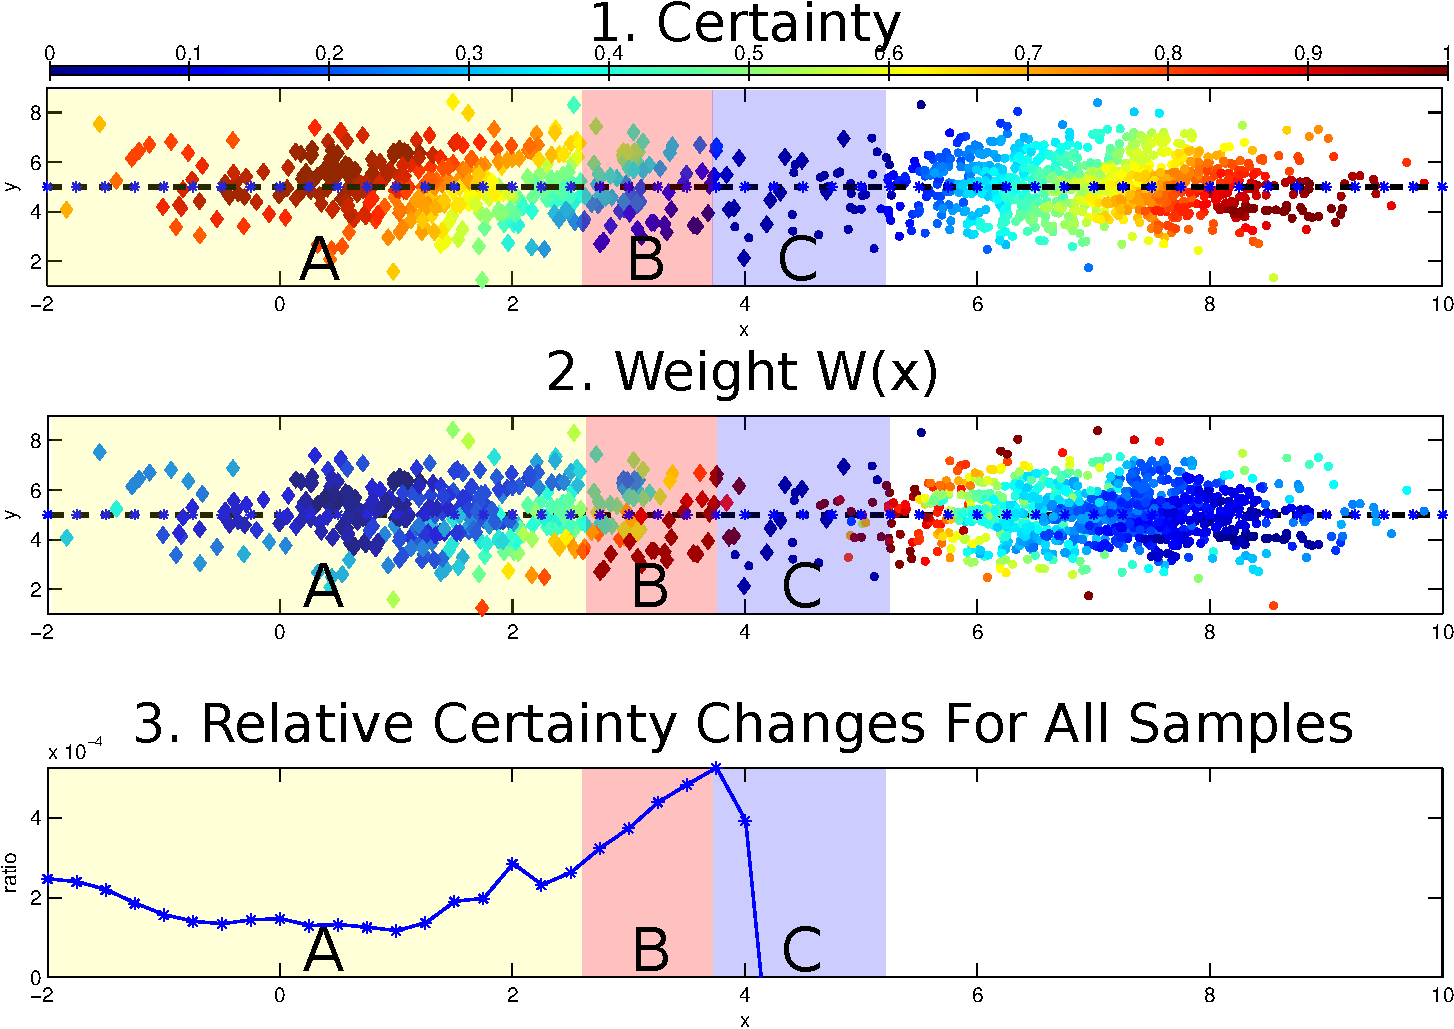
\includegraphics{../Pic/PDF/DemoOfDifferentPosInsertion/UsedInPaper/combined-crop.pdf}}}
\end{tabular}} 
\caption{Demonstration of the proposed approach. In first two figures, diamonds represent minority samples and circles represent majority samples. The positions of synthesized data points are labelled using a star symbol on a horizontal line passing through the center. The x and y axes represent features. In the bottom figure the x axis indicates a location where a sample was added (in correspondence with the first two figures) whereas the y-axis indicates the certainty ratio.}
\label{fig: demoofdiffinsertion} 
\end{figure}

\subsection{Synthesis of New Data}
\label{sec: synthesis of new data}
\textcolor{red}{Simply generating new samples by duplicating minority samples will not guarantee a performance enhancement in resulting dataset. On one hand, just simply add duplicating samples does not increase sample coverage in feature space, therefore seldom information is introduced to the minority class. So it causes a very little change to the decision region of the minority class. On the other hand, adversely, duplicating samples could possibly exert an negative impact to the minority class due to overfitting of tightly aggregated samples in local area.}

\textcolor{red}{In order to increase sample coverage in feature space while avoid overfitting, SMOTE generates a new sample using a linear interpolation on a line segment between a selected seed and one of its nearest neighbors. We employ interpolation to obtain a new sample in the proposed approach as well, but we extend the interpolation step in SMOTE to one that is more general. In the proposed approach, the number of samples used in interpolation is no longer limited to two. In fact, the interpolation of the proposed approach is done in a simplex\footnote{In geometry, a simplex is a generalization of the notion of a triangle or tetrahedron to arbitrary dimensions. For example, a 1-simplex is a line segment, a 2-simplex is a triangle and a 3-simplex is a tetrahedron} composed of a selected seed sample and its neighbors. This is based on a consideration that in a high dimensional dataset, generating samples on a hyper line segment as SMOTE will make us highly likely face the same problems of duplicating data we just talked above.}  

\textcolor{red}{Suppose, there is a set of vertices composing a simplex $S=\{x_1, x_2, \dots, x_v\}$, $x_1, x_2, \dots, x_v \in \mathfrak{R}^m$, where $x_1$ is a seed sample and all other samples in $S$ are its randomly chosen nearest neighbors. $v$ is the number of vertices of a simplex. To guarantee the existence of this simplex, it has to be true that $v\leq m+1$. Actually, our interpolation schema treats the case the same when $S$ is happen not to be a simplex. However, it is worth noting that this case is very unlikely to happen, for example, it is extremely rate to choose three collinear points in a 2 dimensional space given a face that samples in the minority class is very sparse. A new sample $x_{new}$ is going to be generated by interpolating all vertices of $S$. A desire distribution of $x_{new}$ inside the space of $S$ is an uniform distribution. However, naively selecting normalized random weights for each vertices will not result in an expected distribution \cite{SNA:04}. We thus implement an algorithm proposed in \cite{SNA:04} which is able to uniformly and randomly selecting a point from a simplex. For the selection of value of $v$, please refer to Section \ref{sec: results}.}

\section{Theoretical Guarantee Over SMOTE}
Several existing approaches claim handling imbalanced learning better than SMOTE. Such claims are normally validated using empirical tests without a theoretical guarantee and in some instances may not extend to new datasets. \textcolor{red}{In this section we provide a theoretical guarantee showing that the proposed approach is expected to work better than SMOTE using training data and will show superior performance of CGMOS in experiment section.}

Let $D=\{(x_j, y_j)\}_{j=1}^n$ be a training dataset. Let $W(D)=\{W(x_i)\}_{i=1}^n$ be the sample weights computed using Eqn. \ref{eqn: weight}. 
\newline
\newline
\textbf{Lemma 1.} \textit{Given a set of weights $\{W(x_i)\}_{i=1}^n$ as defined above and a normalization factor $z$ given by $z=\sum_{i=1}^n W(x_i)$, it must be that $\sum_{i=1}^n W(x_i)^2 \geq \frac{z^2}{n}$.}
\newline
\newline
\textbf{Proof}
Let $W$ be an n-dimensional vector whose elements are $W(x_i)$. Let $I$ be an n-dimensional vector whose elements are all 1. Using the Cauchy-Schwarz inequality we have: $|W\cdot I|\leq \|W\|\cdot\|I\|$. Thus, $|\sum_{i=1}^n W(x_i)|\leq \sqrt{\sum_{i=1}^n W(x_i)^2 }\sqrt{n}$ using the fact that $\sum_{i=1}^n W(x_i)=z$, we thus have $\sum_{i=1}^n W(x_i)^2 \geq \frac{z^2}{n}$.  $\;\;\;\blacksquare$
\newline
\newline
\noindent\textbf{Definition 3. (Addition likelihood Ratio)} Let $\theta$ denote the non-parametric likelihood estimate $P(x_j|l)$, $l\in \{l_{\mbox{mjr}}, l_{\mbox{mnr}}\}$ before a new sample $x_i$ is added, and $\theta'$ denote the non-parametric likelihood estimate after the new sample is added. The addition likelihood ratio $r_{+i}(y_j|x_j)$ of example $x_j$ by adding data to $x_i$ location is defined as the ratio between the likelihood estimate after the new addition and the likelihood estimate before the new addition: 
\begin{equation}
r_{+i}(y_j|x_j) \equiv P(y_j|x_j ; \theta') / P(y_j|x_j; \theta).
\label{eqn. likelihoodratio}
\end{equation}
\newline
\textcolor{red}{\noindent \textbf{Lemma 2.} \textit{The addition likelihood ratio $r_{+i}(y_j|x_j)$ is related to the certainty ratio $R_{+i}(y_j|x_j)$ by: }
\begin{equation}
r_{+i}(y_j|x_j)=\exp({R_{+i}(y_j|x_j)}).
\end{equation}}

\textcolor{red}{\noindent\textbf{Proof} According to the definition of the certainty, we have that $C_{+i}(y_j|x_j)=P(y_j|x_j; \theta')$ and $C(y_j|x_j; \theta)=P(y_j|x_j; \theta)$. Then $P(y_j|x_j; \theta')=r_{+i}(y_j|x_j) P(y_j|x_j; \theta)$ according to the definition of likelihood ratio. Given Eqn. \ref{eqn: relative diff}, we have that $R_{+i}(y_j | x_j)=\log\frac{r_{+i}(y_j|x_j) P(y_j | x_j; \theta)}{P(y_j |x_j; \theta)}$.  By simplifying this equation, we thus have 
\begin{equation}
r_{+i}(y_j|x_j)=\exp(R_{+i}(y_j|x_j)). \;\;\;\blacksquare
\end{equation}
The addition likelihood ratio defined in Eqn. \ref{eqn. likelihoodratio} measures the gain in adding a new point, where higher gains are desired. Note that while the gain is normally close to 1 it may be bigger or smaller than 1.
\newline}

\textcolor{red}{\noindent\textbf{Definition 4. (Likelihood of Non-parametric Estimate)} Given the variables $\theta$ of non-parametric likelihood estimate $P(y_j|x_j; \theta)$, $(x_j, y_j)\in D$, the likelihood of the non-parametric estimate on a dataset $D$ is defined as:}

\textcolor{red}{
\begin{equation}
\mathcal{L}(\theta; D)=\prod_{j=1}^n P(y_j|x_j; \theta)
\end{equation}}

\textcolor{red}{\noindent \textbf{Theorem 1.} \textit{Assuming that one sample $(x_i, y_i)\in D$ is chosen for interpolation and the resulting variables of non-parametric model are $\theta'$, CGMOS will choose a sample whose resulting expected likelihood is larger than or equal to the one resulting from a sample chosen by SMOTE.}
\newline}

\textcolor{red}{\noindent\textbf{Proof} Assume the posterior of each sample generated by the original dataset is given by $P(y_j|x_j;\theta)$, for all $(x_j, y_j)\in D$. The variables of the non-parametric model estimate become from $\theta$ to $\theta'$ when a new data sample $(x_i, y_i)$ is added and the posterior of each sample $(x_j, y_j)$ is changed by the addition likelihood ratio $r_{+i}(y_j|x_j)$ as defined in Eqn.\ref{eqn. likelihoodratio}. Using this notation, the likelihood $\mathcal{L}(\theta; D)=\prod_{j=1}^n P(y_j|x_j; \theta)$ after adding the sample becomes to:
\begin{equation}
\mathcal{L}(\theta_{+i}; D)=\prod_{j=1}^n P(y_j|x_j; \theta) \cdot r_{+i}(y_j|x_j).
\end{equation}
By converting the likelihood to its log form, we have:
\begin{align}
\log \mathcal{L}(\theta_{+i}; D)=&\log{\prod_{j=1}^n P(y_j|x_j; \theta)} +\sum_{j=1}^n \log(r_{+i}(y_j|x_j))\\
                            =&\mathcal{L}(\theta; D) + \sum_{j=1}^n \log(r_{+i}(y_j|x_j)).
\end{align}
Using Lemma 2:
\begin{align}
\log{\mathcal{L}(\theta'; D)}=&\log{\mathcal{L}(\theta; D)} + \sum_{j=1}^n \log(\exp(R_{+i}(y_j|x_j)))\\
							=&\log{\mathcal{L}(\theta; D)} + \sum_{j=1}^n R_{+i}(y_j|x_j).
\end{align}
which can be further simplified using Eqn.\ref{eqn: weight}:
\begin{equation}
\log{\mathcal{L}(\theta'; D)} = \log\mathcal{L}(\theta; D) + nW(x_i) - n
\end{equation}
For CGMOS the expected likelihood is given by:
\begin{align}
E_{c}\equiv E[\log\mathcal{L}(\theta'; D)]=&E[\log\mathcal{L}(\theta; D)] + nE[W(x_i)] - n
\end{align}
Since the term inside the first expectation is a constant, we have:
\begin{equation}
E_{c} = \log\mathcal{L}(\theta; D) + nE(W(x_i))-n
\end{equation}
Given the normalization factor $z$ of $W(x_i)$:
\begin{align}
E_{c} =& \log\mathcal{L}(\theta; D) + nE(W(x_i)) - n\\
		  =& \log\mathcal{L}(\theta; D) + n \sum_{i=1}^n W(x_i)\frac{W(x_i)}{z} - n\\
		  =& \log\mathcal{L}(\theta; D) + \frac{n}{z} \sum_{i=1}^n W(x_i)^2 -n
\end{align}
For SMOTE the expected likelihood is given by:
\begin{align}
E_{s}\equiv E[\log\mathcal{L}(\theta'; D)]=&E[\log\mathcal{L}(\theta; D)] + nE[W(x_i)]-n
\end{align}
Since SMOTE uniformly randomly draws sample for interpolation, we have:
\begin{align}
E_{s}=&E[\log\mathcal{L}(\theta; D)] + n\sum_{i=1}^n \frac{W(x_i)}{n} - n\\
	 =&\log\mathcal{L}(\theta; D) + z - n
\end{align}
Using Lemma 1:
\begin{equation}
E_{c} = \log\mathcal{L}(\theta; D) + \frac{n}{z} \sum_{i=1}^n W(x_i)^2 - n\geq \log\mathcal{L}(\theta; D) + z -n = E_s
\end{equation}}

\subsection{Time complexity}
\textcolor{red}{At first glance, the computation cost of $W(x_i)$ is a bottleneck as the computation of $W(x_i)$ is quadratic in the number of examples and has to be done for all samples which results in a cubic complexity. However, the computation of $W(x_i)$ can be done in linear time by updating the posterior $P(l|x_j)$, $l\in \{l_{\mbox{mjr}}, l_{\mbox{mnr}}\}$ instead of recomputing it from scratch. We begin by recording a pairwise distance matrix and the original posterior for all samples in the dataset. The updating of $P(l|x_j)$ can be done in a linear time, and overall, the proposed approach has a $O(n^2)$ time complexity.} 

\section{Results and Discussion}
\label{sec: results}
\textcolor{red}{In this section, we evaluate the performance of the proposed CGMOS. According to a survey of \cite{HH:09}, there are mainly three groups of methods addressing imbalanced learning: sampling methods, cost sensitive methods and kernel methods. Since the proposed CGMOS belongs to the group of the sampling methods, we focus our evaluations on methods from the same group. It is worth noting that the resulting dataset of sampling methods can be used by methods in the other two groups which will further boost the performance.}

\subsection{Datasets}
\subsubsection{Artificial Datasets}
\textcolor{red}{Artificial datasets are created and tested to help us better show and understand the advantage of CGMOS over all other competitors. To better simulate datasets with different imbalance ratio, we fix the amount of majority samples to 1000 and adjust the amount of minority data. Thus three groups of datasets with imbalance ratio ($r_{imb}=0.025, 0.05, 0.1$) are generated in 2D space. To generate data in one dataset, we assume both majority and minority class follow a normal distribution $\mathcal{N}(\mu_{\{\mbox{mjr}, \mbox{mnr}\}}, \Sigma)$ where $\Sigma$ is an identity matrix. Then for datasets in each of the three groups, we adjust the distance between $\mu_{\mbox{mjr}}$ and $\mu_{\mbox{mnr}}$ indicated by $d_{\mu}$ to generate datasets with different difficulties of classification. $d_{\mu}=4$ and $d_{\mu}=2.5$ are used which results in 6 artificial datasets in total. We indeed tried datasets with some other distributions such as uniform distribution in our tests and the results are very similar to the ones we show in this paper.}

\subsubsection{Real-world Datasets}
30 real-world datasets were randomly chosen from the UCI machine learning repository \cite{Lichman:2013} for empirical testing of CGMOS. Most of the datasets were released within the past 10 years. As some of the datasets contain samples of more than two classes, we convert such datasets to a binary classification problem by keeping the class with the least data and merging all other classes. A summary of the test collections is provided in Table \ref{tab: realdata}.


\begin{table}[]
\begin{center}
\scalebox{1.0}
{
\begin{tabular}{!{\VRule[1.5pt]}l!{\VRule[1.5pt]}l|l|l|l!{\VRule[1.5pt]}}
\specialrule{1.5pt}{0pt}{0pt} 
 & \textbf{S\#} & \textbf{F\#} & \textbf{R} & \textbf{Year} \\
 \specialrule{1.5pt}{0pt}{0pt} 
\textbf{BankMarket} & 45211 & 17 & 0.13 & 2012 \\ \hline
\textbf{BloodTransService} & 748 & 5 & 0.31 & 2008 \\ \hline
\textbf{BreastCancer} & 400 & 9 & 0.53 & 1988 \\ \hline
\textbf{BreastTissue} & 106 & 10 & 0.15 & 2010 \\ \hline
\textbf{CarEvaluation} & 1730 & 6 & 0.04 & 1997 \\ \hline
\textbf{Cardiotocography} & 2126 & 23 & 0.09 & 2010 \\ \hline
\textbf{CharacterTrajectories} & 2860 & 3 & 0.04 & 2008 \\ \hline
\textbf{Chess} & 3198 & 22 & 0.91 & 1989 \\ \hline
\textbf{ClimateSimulation} & 540 & 18 & 0.09 & 2013 \\ \hline
\textbf{ContraceptiveMethod} & 1474 & 9 & 0.29 & 1997 \\ \hline
\textbf{Fertility} & 100 & 10 & 0.14 & 2013 \\ \hline
\textbf{Haberman} & 306 & 3 & 0.36 & 1999 \\ \hline
\textbf{ILPD} & 580 & 10 & 0.4 & 2012 \\ \hline
\textbf{ImgSegmentation} & 2310 & 19 & 0.17 & 1990 \\ \hline
\textbf{Leaf} & 342 & 16 & 0.24 & 2014 \\ \hline
\textbf{Libras} & 360 & 91 & 0.07 & 2009 \\ \hline
\textbf{MultipleFeatures} & 2000 & 649 & 0.11 & 1998 \\ \hline
\textbf{ParkinsonSpeech} & 1040 & 26 & 0.02 & 2014 \\ \hline
\textbf{PlanningRelax} & 182 & 13 & 0.4 & 2012 \\ \hline
\textbf{QSAR} & 1055 & 41 & 0.51 & 2013 \\ \hline
\textbf{SPECT} & 268 & 22 & 0.26 & 2001 \\ \hline
\textbf{SPECTF} & 134 & 44 & 0.26 & 2001 \\ \hline
\textbf{SeismicBumps} & 2584 & 19 & 0.07 & 2013 \\ \hline
\textbf{Statlog} & 2310 & 19 & 0.17 & 1990 \\ \hline
\textbf{SteelPlatesFaults} & 1941 & 27 & 0.03 & 2010 \\ \hline
\textbf{TAEvaluation} & 151 & 5 & 0.49 & 1997 \\ \hline
\textbf{UserKnowledge} & 403 & 5 & 0.1 & 2013 \\ \hline
\textbf{Vertebral} & 310 & 6 & 0.48 & 2011 \\ \hline
\textbf{WholesaleCustomers} & 440 & 8 & 0.48 & 2014 \\ \hline
\textbf{Yeast} & 1484 & 8 & 0.04 & 1996 \\
\specialrule{1.5pt}{0pt}{0pt} 
\end{tabular}
}
\end{center}
\caption{Summary of the datasets used in our experiments, where S\#, F\#, and R stand for the number of samples, the number of features, and imbalance ratio (defined as \#minority/\#majority).}
\label{tab: realdata}
\end{table}

\subsection{Compared Approaches}
According to a survey of imbalanced learning \cite{HH:09}, there are mainly three groups of methods addressing imbalanced learning: sampling methods, cost sensitive methods, and kernel methods. The proposed CGMOS belongs to the sampling group. Thus, we compare CGMOS to five other oversampling methods in this group: SMOTE\cite{CNV:02}, Borderline-SMOTE\cite{HH:05}, ADASYN\cite{HH:08}, MWMOTE\cite{barua2014mwmote} and RAMOBoost\cite{chen2010ramoboost}. Since oversampling by duplication is broadly used in many applications as a baseline, we add it to our evaluation as well. To demonstrate the improvement of these oversampling strategies, we include in the comparison raw data with no oversampling. It should be noted that sampling methods are often combined with cost sensitive methods and kernel methods to further boost learning. \cite{chawla2004editorial}\cite{chawla2003smoteboost}\cite{guo2004learning}.

\subsection{Base classifiers}
We match the compared classifiers to classifiers used in other SMOTE extension evaluations. Six well-known classifiers are tested in our experiments: Bayesian classifier based on kernel density estimation described in Section \ref{sec: problem formulation} (b-kde), K nearest neighbors classifier (knn), support vector machine classifier using RBF kernel (svm), neural network (nn) with one hidden layer, a random forest implementing the C4.5 decision tree \cite{Quinlan:1993} (rf), and Adaboost.M1 \cite{fy:1996}. All hyper-parameters of the classifiers tested were determined by cross validation to ensure the best performance of each method.

\begin{figure}[ht]
\centerline{ %
\begin{tabular}{cc}
\resizebox{0.23\textwidth}{!}{\rotatebox{0}{ 
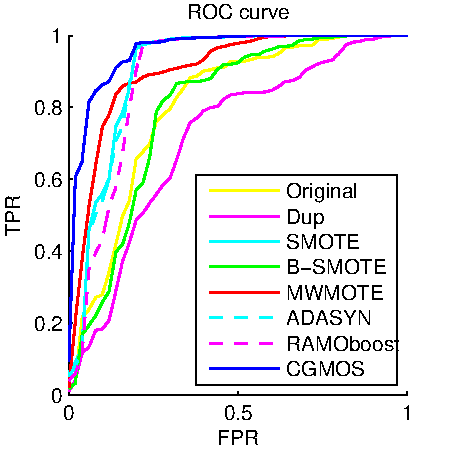
\includegraphics{../Pic/PDF/SyntheticData/syn_ratio_0.025/4.pdf}}}
&
\resizebox{0.23\textwidth}{!}{\rotatebox{0}{ 
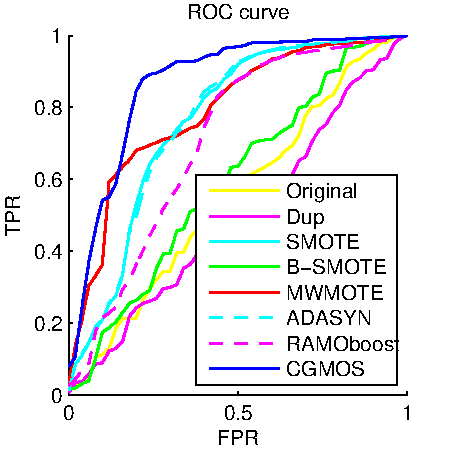
\includegraphics{../Pic/PDF/SyntheticData/syn_ratio_0.025/6.pdf}}}
\\
ratio=0.025, d=4 & ratio=0.025, d=2.5
\\
\resizebox{0.23\textwidth}{!}{\rotatebox{0}{ 
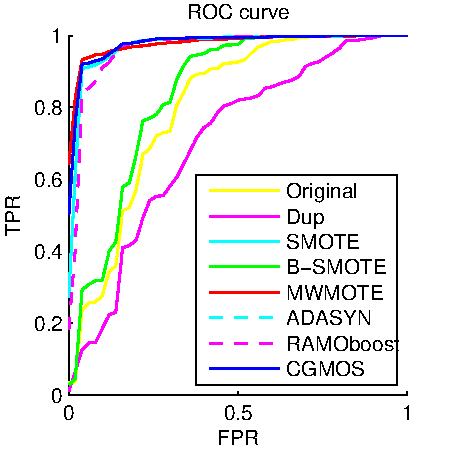
\includegraphics{../Pic/PDF/SyntheticData/syn_ratio_0.05/4.pdf}}}
&
\resizebox{0.23\textwidth}{!}{\rotatebox{0}{ 
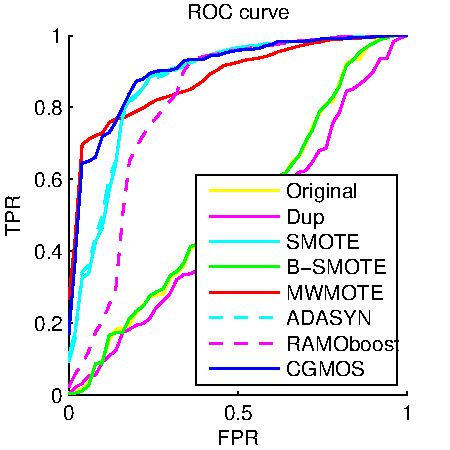
\includegraphics{../Pic/PDF/SyntheticData/syn_ratio_0.05/6.pdf}}}
\\
ratio=0.05, d=4 & ratio=0.05, d=2.5
\\
\resizebox{0.23\textwidth}{!}{\rotatebox{0}{ 
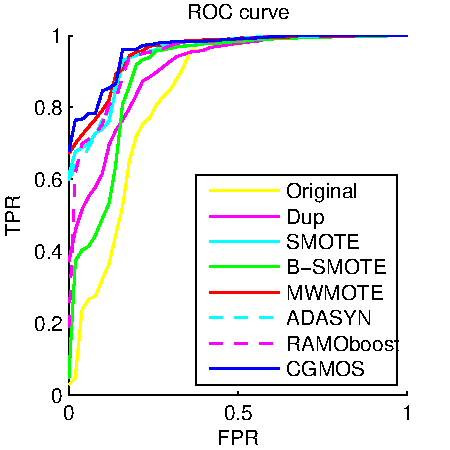
\includegraphics{../Pic/PDF/SyntheticData/syn_ratio_0.1/4.pdf}}}
&
\resizebox{0.23\textwidth}{!}{\rotatebox{0}{ 
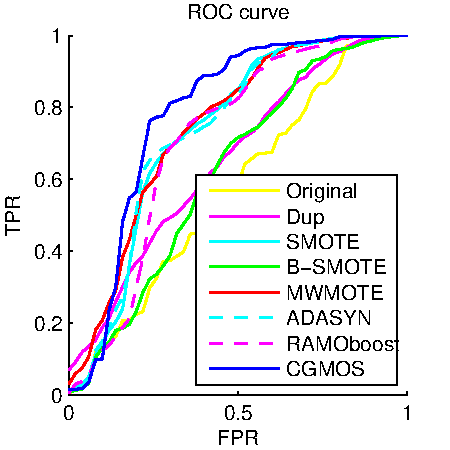
\includegraphics{../Pic/PDF/SyntheticData/syn_ratio_0.1/6.pdf}}}
\\
ratio=0.1, d=4 & ratio=0.1, d=2.5
\end{tabular}} 
\caption{ROC curves of the artificial datasets classification results using b-kde classifier. In total, results of 6 datasets are shown in the above figures.}
\label{fig: synthetic roc} 
\end{figure}

\subsection{Evaluation metric}
Finding an appropriate evaluation metric for different tasks is challenging, since different evaluation metrics are designed for different purposes. The datasets used in this paper cover topics ranging from financial applications to medical treatments. To achieve a general evaluation and avoid bias, we follow the method in \cite{CNV:02}\cite{HH:05}\cite{HH:08}\cite{barua2014mwmote}\cite{chen2010ramoboost} and use different metrics to evaluate the performance of the proposed CGMOS oversampling algorithm.

\textcolor{red}{Among these evaluation metrics, the most frequently adopted ones are $Precision$ and $Recall$ when the focus of evaluation is focus on one specific class such as problems in text classification, information extraction, natural language processing and bioinformatics. In these areas of application the number of examples belonging to one class is often substantially lower than the overall number of examples, which basically are imbalance learning problems. $Precision$ and $Recall$ are defined as:}

\begin{align*}
Precision &= \frac{TP}{(TP + FP)}\\
Recall &= \frac{TP}{(TP+FN)}  
\end{align*}

\textcolor{red}{However, these two metrics share an inverse relationship between each other. A quick inspection on the $Precision$ and $Recall$ formulas readily yields that solely use each of these two metrics only provide a limit view of an algorithm under test. As $Recall$ provides no insight to how many examples are incorrectly labeled as positive and $Precision$ cannot assert how many positive examples are labeled incorrectly. Specifically, the $\fscore$ combines $Precision$ and $Recall$ as measure of the effectiveness of classification in terms of a ration of the weighted importance on either $Recall$ or $Precision$, which is defined as:}
\begin{align*}
\fscore = \frac{(1+\beta^2)\cdot Precision \cdot Recall}{(\beta^2\cdot Precision)+ Recall}.
\end{align*}
We use $\beta=1$ to treat $Precision$ and $Recall$ equally in all evaluations. As a result, $\fscore$ provides more insight into the functionality of a classifier. We also compute $Gscore$ which is the geometric mean of $Precision$ and $Recall$ and is able to evaluate the degree of inductive bias in terms of a ratio of positive accuracy and negative accuracy \cite{HH:09}.

\begin{align*}
\gscore=\sqrt{Precision \cdot Recall}
\end{align*}

As both $\fscore$ and $\gscore$ concentrate their measures on one class (positive examples) \cite{sokolova2006beyond}, to have a general way of comparing our test results, we switched the labeling of positive examples between the majority and minority classes when computing the $\fscore$ and $\gscore$. Thus, we show $\fscore$ and $\gscore$ for the majority and the minority classes separately.

Although, both $\fscore$ and $\gscore$ are common evaluation metrics, they capture a single point of performance. Thus, we employ ROC curves \cite{fawcett2004roc}\cite{fawcett2006introduction}\cite{mohri2005confidence} in the evaluation.

ROC curves show relative trade-off between benefit (true positive) and cost (false positive). A useful property that makes ROC curves a good metric in imbalanced learning lies in the facts that ROC curves are insensitive to changes in class distribution. This makes easier comparing the performance of models trained by dataset oversampled by different algorithms. We also compute area under the ROC curve (AUC) for each evaluated method.
 
 
\subsection{Results}
\subsubsection{Experiments on Artificial Datasets}
\textcolor{red}{For all artificial datasets in the test, all oversampling algorithms only add synthetic data to the minority class to match the majority class in the training set and the same partition of the datasets were used for all oversampling algorithms. We use b-kde classifier for all classification tasks in this test. 10 rounds of 10-folds cross-validation were performed. We compute an average performance of all experiments in the evaluation. A summary of all the results are shown in Table \ref{tab: results_synthetic_data}. We show results of $Precision$, $Recall$, $\fscore$ and $\gscore$ for the majority and minority classes separately to give a more clear insight about how the majority and minority classes are affected by each methods in the classification. In Table \ref{tab: results_synthetic_data}, from up to down, results are organized to 6 chunks corresponding to 6 artificial datasets in total. The imbalance ratio $r_{imb}$ and the distance $d_{\mu}$ between centers of the majority and minority classes are shown in the front of each chunk to indicate the beginning of the results.}

\textcolor{red}{Some patterns can be easily seen from the results in Table \ref{tab: results_synthetic_data}. In all cases, the classifiers trained using original dataset misclassified the minority class all the time. This is because without oversampling the minority class in the original dataset, the b-kde classifier try to compromise every single sample of the majority class, thus push and mistakenly expand the decision boundary towards the minority class.} 

\textcolor{red}{Some interesting results are given by Dup in the table, where almost all minority samples are misclassified. This basically means that the new samples generated by duplicating does not help expand the decision boundary on the minority class side, which is due to the fact that few helpful information is added to the dataset by just copying the original samples. In fact, it could be seen from the ROC graphs in Figure \ref{fig: synthetic roc} that for artificial dataset with $r_{imb}= 0.025, d_{\mu}=2.5$ and dataset with $r_{imb}=0.05, d_{\mu}=2.5$, the performances of the Original and Dup are no better than results produced by just guessing and the same thing call be told for B-SMOTE in these two ROC graphs. }

\textcolor{red}{For methods MWMOTE and RAMOboost in the Table \ref{tab: results_synthetic_data} whose results generally have much higher $Precision$ value than $Recall$ for the minority class, the phenomenons can be explained by a fact that these two methods are relatively conservative and they generally try to avoid the risk area as we illustrate in Figure \ref{fig: demoofdiffinsertion} when synthesizing new samples. Thus, the added samples will not help classifying minority samples that are very close to the majority class. On the contrary, the behaviors of SMOTE and ADASYN are more defensive in terms of the way how they oversampling the minority class. SMOTE basically adds more samples in a random manner and ADASYN prefers putting new samples along boundary regions, so they all are highly likely to synthesize more samples in the risk areas which in turn has to sacrifice the classification performance of the majority class to win a slightly better $Recall$ results for the minority class.} 

\textcolor{red}{Compared with these methods, CGMOS achieves the best results in tests of all 6 datasets. It could be seen from Figure \ref{fig: synthetic roc} that although CGMOS just slightly win all other competitors for datasets which are relatively easier to classify, the ROC curves of CGMOS almost dominate the ROC graphs for the datasets where the classification difficulties are increased. The credit should be given to the CGMOS's ability of always adaptively synthesizing samples in places where the certainty of the resulting dataset can be almost maximized in classification.}

\textcolor{red}{It also could be easily seen from the results in Table \ref{tab: results_synthetic_data} and the ROC graphs in Figure \ref{fig: synthetic roc} that when the imbalance ratio $r_{imb}$ is lower, it is harder to get the minority class correctly classified. Similarly, there are more misclassified cases when the centers of the majority class and minority class move closer. Based on this observation, we can compute the standard deviation of AUC of all datasets from each method, which in turn can be used to relatively show the stability of each method. CGMOS has the standard deviation of $0.076$ which is the smallest when compared to all the other methods (Original=$0.146$, Dup=$0.165$, SMOTE=$0.097$, B-SMOTE=$0.153$, MWMOTE=$0.098$, ADASYN=$0.097$ and RAMOboost=$0.112$). Thus CGMOS is more robust and stable to use as compared with all the other competitors.}

\begin{table*}[]
\begin{center}
\scalebox{1.0}{
\begin{tabular}{lc!{\VRule[1.5pt]}c|c|c|c!{\VRule[1.5pt]}c|c|c|c!{\VRule[1.5pt]}}
\Cline{1.5pt}{3-10}
 & \textbf{} & \multicolumn{4}{c!{\VRule[1.5pt]}}{\textbf{Minority}} & \multicolumn{4}{c!{\VRule[1.5pt]}}{\textbf{Majority}} \\ \Cline{1.5pt}{2-10} 
\multicolumn{1}{l!{\VRule[1.5pt]}}{} & \textbf{AUC} & \textbf{Precision} & \textbf{Recall} & \textbf{Fscore} & \textbf{Gscore} & \textbf{Precision} & \textbf{Recall} & \textbf{Fscore} & \textbf{Gscore} \\
\specialrule{1.5pt}{0pt}{0pt}
\multicolumn{1}{!{\VRule[1.5pt]}l!{\VRule[1.5pt]}}{\textbf{$r_{imb}=0.025$, $d_{\mu}=4$}} &  & \multicolumn{4}{c!{\VRule[1.5pt]}}{} & \multicolumn{4}{c!{\VRule[1.5pt]}}{} \\
\specialrule{1.5pt}{0pt}{0pt}
\multicolumn{1}{!{\VRule[1.5pt]}l!{\VRule[1.5pt]}}{\textbf{Original}} & 0.793 & 0.000 & 0.000 & 0.000 & 0.000 & 0.952 & 1.000 & 0.976 & 0.976 \\ \hline
\multicolumn{1}{!{\VRule[1.5pt]}l!{\VRule[1.5pt]}}{\textbf{Dup}} & 0.704 & 0.000 & 0.000 & 0.000 & 0.000 & 0.952 & 1.000 & 0.976 & 0.976 \\ \hline
\multicolumn{1}{!{\VRule[1.5pt]}l!{\VRule[1.5pt]}}{\textbf{SMOTE}} & 0.890 & 0.778 & \textbf{0.700} & \textbf{0.737} & \textbf{0.738} & \textbf{0.985} & 0.990 & \textbf{0.988} & \textbf{0.988} \\ \hline
\multicolumn{1}{!{\VRule[1.5pt]}l!{\VRule[1.5pt]}}{\textbf{B-SMOTE}} & 0.785 & 0.000 & 0.000 & 0.000 & 0.000 & 0.952 & 1.000 & 0.976 & 0.976 \\ \hline
\multicolumn{1}{!{\VRule[1.5pt]}l!{\VRule[1.5pt]}}{\textbf{MWMOTE}} & 0.893 & \textbf{0.864} & 0.380 & 0.528 & 0.573 & 0.970 & \textbf{0.994} & 0.983 & 0.983 \\ \hline
\multicolumn{1}{!{\VRule[1.5pt]}l!{\VRule[1.5pt]}}{\textbf{ADASYN}} & 0.886 & 0.745 & \textbf{0.700} & 0.722 & 0.722 & 0.985 & 0.988 & 0.987 & 0.987 \\ \hline
\multicolumn{1}{!{\VRule[1.5pt]}l!{\VRule[1.5pt]}}{\textbf{RAMOboost}} & 0.872 & 0.823 & 0.608 & 0.699 & 0.707 & 0.981 & 0.992 & 0.987 & 0.987 \\ \hline
\multicolumn{1}{!{\VRule[1.5pt]}l!{\VRule[1.5pt]}}{\textbf{CGMOS}} & \textbf{0.947} & 0.838 & 0.620 & 0.713 & 0.721 & 0.981 & \textbf{0.994} & \textbf{0.988} & \textbf{0.988} \\
\specialrule{1.5pt}{0pt}{0pt}
\multicolumn{1}{!{\VRule[1.5pt]}l!{\VRule[1.5pt]}}{\textbf{$r_{imb}=0.025$, $d_{\mu}=2.5$}} &  & \multicolumn{4}{c|}{} & \multicolumn{4}{c!{\VRule[1.5pt]}}{} \\
\specialrule{1.5pt}{0pt}{0pt}
\multicolumn{1}{!{\VRule[1.5pt]}l!{\VRule[1.5pt]}}{\textbf{Original}} & 0.541 & 0.000 & 0.000 & 0.000 & 0.000 & 0.952 & \textbf{1.000} & \textbf{0.976} & \textbf{0.976} \\ \hline
\multicolumn{1}{!{\VRule[1.5pt]}l!{\VRule[1.5pt]}}{\textbf{Dup}} & 0.488 & 0.000 & 0.000 & 0.000 & 0.000 & 0.952 & \textbf{1.000} & \textbf{0.976} & \textbf{0.976} \\ \hline
\multicolumn{1}{!{\VRule[1.5pt]}l!{\VRule[1.5pt]}}{\textbf{SMOTE}} & 0.745 & 0.250 & 0.400 & 0.308 & 0.316 & \textbf{0.969} & 0.940 & 0.954 & 0.954 \\ \hline
\multicolumn{1}{!{\VRule[1.5pt]}l!{\VRule[1.5pt]}}{\textbf{B-SMOTE}} & 0.584 & 0.000 & 0.000 & 0.000 & 0.000 & 0.952 & \textbf{1.000} & \textbf{0.976} & \textbf{0.976} \\ \hline
\multicolumn{1}{!{\VRule[1.5pt]}l!{\VRule[1.5pt]}}{\textbf{MWMOTE}} & 0.782 & 0.303 & 0.200 & 0.241 & 0.246 & 0.961 & 0.977 & 0.969 & 0.969 \\ \hline
\multicolumn{1}{!{\VRule[1.5pt]}l!{\VRule[1.5pt]}}{\textbf{ADASYN}} & 0.755 & 0.319 & \textbf{0.460} & 0.377 & 0.383 & 0.972 & 0.951 & 0.962 & 0.962 \\ \hline
\multicolumn{1}{!{\VRule[1.5pt]}l!{\VRule[1.5pt]}}{\textbf{RAMOboost}} & 0.703 & 0.230 & 0.280 & 0.252 & 0.254 & 0.964 & 0.953 & 0.958 & 0.958 \\ \hline
\multicolumn{1}{!{\VRule[1.5pt]}l!{\VRule[1.5pt]}}{\textbf{CGMOS}} & \textbf{0.857} & \textbf{0.438} & 0.280 & \textbf{0.342} & \textbf{0.412} & \textbf{0.969} & 0.981 & \textbf{0.975} & \textbf{0.975} \\
\specialrule{1.5pt}{0pt}{0pt}
\multicolumn{1}{!{\VRule[1.5pt]}l!{\VRule[1.5pt]}}{\textbf{$r_{imb}=0.05$, $d_{\mu}=4$}} &  & \multicolumn{4}{c|}{} & \multicolumn{4}{c!{\VRule[1.5pt]}}{} \\
\specialrule{1.5pt}{0pt}{0pt}
\multicolumn{1}{!{\VRule[1.5pt]}l!{\VRule[1.5pt]}}{\textbf{Original}} & 0.792 & 0.000 & 0.000 & 0.000 & 0.000 & 0.952 & \textbf{1.000} & 0.976 & 0.976 \\ \hline
\multicolumn{1}{!{\VRule[1.5pt]}l!{\VRule[1.5pt]}}{\textbf{Dup}} & 0.674 & 0.000 & 0.000 & 0.000 & 0.000 & 0.952 & \textbf{1.000} & 0.976 & 0.976 \\ \hline
\multicolumn{1}{!{\VRule[1.5pt]}l!{\VRule[1.5pt]}}{\textbf{SMOTE}} & 0.964 & 0.717 & \textbf{0.760} & 0.738 & 0.738 & 0.988 & 0.985 & 0.987 & 0.987 \\ \hline
\multicolumn{1}{!{\VRule[1.5pt]}l!{\VRule[1.5pt]}}{\textbf{B-SMOTE}} & 0.829 & 0.000 & 0.000 & 0.000 & 0.000 & 0.952 & \textbf{1.000} & 0.976 & 0.976 \\ \hline
\multicolumn{1}{!{\VRule[1.5pt]}l!{\VRule[1.5pt]}}{\textbf{MWMOTE}} & \textbf{0.974} & 0.707 & 0.580 & 0.637 & 0.641 & 0.979 & 0.988 & 0.984 & 0.984 \\ \hline
\multicolumn{1}{!{\VRule[1.5pt]}l!{\VRule[1.5pt]}}{\textbf{ADASYN}} & 0.964 & 0.667 & 0.800 & 0.727 & 0.730 & \textbf{0.990} & 0.980 & 0.985 & 0.985 \\ \hline
\multicolumn{1}{!{\VRule[1.5pt]}l!{\VRule[1.5pt]}}{\textbf{RAMOboost}} & 0.959 & \textbf{0.810} & 0.680 & 0.739 & 0.742 & 0.984 & 0.992 & \textbf{0.988} & \textbf{0.988} \\ \hline
\multicolumn{1}{!{\VRule[1.5pt]}l!{\VRule[1.5pt]}}{\textbf{CGMOS}} & \textbf{0.974} & 0.800 & 0.720 & \textbf{0.758} & \textbf{0.759} & 0.986 & 0.991 & \textbf{0.989} & \textbf{0.989} \\
\specialrule{1.5pt}{0pt}{0pt}
\multicolumn{1}{!{\VRule[1.5pt]}l!{\VRule[1.5pt]}}{\textbf{$r_{imb}=0.05$, $d_{\mu}=2.5$}} &  & \multicolumn{4}{c|}{} & \multicolumn{4}{c!{\VRule[1.5pt]}}{} \\
\specialrule{1.5pt}{0pt}{0pt}
\multicolumn{1}{!{\VRule[1.5pt]}l!{\VRule[1.5pt]}}{\textbf{Original}} & 0.517 & 0.000 & 0.000 & 0.000 & 0.000 & 0.952 & \textbf{1.000} & \textbf{0.976} & \textbf{0.976} \\ \hline
\multicolumn{1}{!{\VRule[1.5pt]}l!{\VRule[1.5pt]}}{\textbf{Dup}} & 0.453 & 0.000 & 0.000 & 0.000 & 0.000 & 0.952 & \textbf{1.000} & \textbf{0.976} & \textbf{0.976} \\ \hline
\multicolumn{1}{!{\VRule[1.5pt]}l!{\VRule[1.5pt]}}{\textbf{SMOTE}} & 0.865 & 0.500 & \textbf{0.380} & 0.423 & 0.427 & \textbf{0.969} & 0.981 & \textbf{0.975} & \textbf{0.975} \\ \hline
\multicolumn{1}{!{\VRule[1.5pt]}l!{\VRule[1.5pt]}}{\textbf{B-SMOTE}} & 0.517 & 0.000 & 0.000 & 0.000 & 0.000 & 0.952 & \textbf{1.000} & \textbf{0.976} & \textbf{0.976} \\ \hline
\multicolumn{1}{!{\VRule[1.5pt]}l!{\VRule[1.5pt]}}{\textbf{MWMOTE}} & 0.879 & 0.351 & 0.260 & 0.299 & 0.302 & 0.964 & 0.976 & 0.970 & 0.970 \\ \hline
\multicolumn{1}{!{\VRule[1.5pt]}l!{\VRule[1.5pt]}}{\textbf{ADASYN}} & 0.861 & \textbf{0.539} & 0.353 & \textbf{0.426} & \textbf{0.436} & 0.967 & 0.980 & 0.974 & 0.974 \\ \hline
\multicolumn{1}{!{\VRule[1.5pt]}l!{\VRule[1.5pt]}}{\textbf{RAMOboost}} & 0.786 & 0.516 & 0.320 & 0.395 & 0.406 & 0.967 & 0.985 & \textbf{0.976} & \textbf{0.976} \\ \hline
\multicolumn{1}{!{\VRule[1.5pt]}l!{\VRule[1.5pt]}}{\textbf{CGMOS}} & \textbf{0.896} & 0.487 & \textbf{0.380} & \textbf{0.427} & 0.430 & \textbf{0.969} & 0.980 & \textbf{0.975} & \textbf{0.975} \\
\specialrule{1.5pt}{0pt}{0pt}
\multicolumn{1}{!{\VRule[1.5pt]}l!{\VRule[1.5pt]}}{\textbf{$r_{imb}=0.1$, $d_{\mu}=4$}} &  & \multicolumn{4}{c|}{} & \multicolumn{4}{c!{\VRule[1.5pt]}}{} \\
\specialrule{1.5pt}{0pt}{0pt}
\multicolumn{1}{!{\VRule[1.5pt]}l!{\VRule[1.5pt]}}{\textbf{Original}} & 0.827 & 0.000 & 0.000 & 0.000 & 0.000 & 0.952 & \textbf{1.000} & 0.976 & 0.976 \\ \hline
\multicolumn{1}{!{\VRule[1.5pt]}l!{\VRule[1.5pt]}}{\textbf{Dup}} & 0.905 & \textbf{1.000} & 0.100 & 0.182 & 0.316 & 0.957 & \textbf{1.000} & 0.978 & 0.978 \\ \hline
\multicolumn{1}{!{\VRule[1.5pt]}l!{\VRule[1.5pt]}}{\textbf{SMOTE}} & 0.945 & 0.674 & 0.660 & 0.667 & \textbf{0.667} & \textbf{0.983} & 0.984 & \textbf{0.983} & \textbf{0.983} \\ \hline
\multicolumn{1}{!{\VRule[1.5pt]}l!{\VRule[1.5pt]}}{\textbf{B-SMOTE}} & 0.891 & 0.706 & 0.240 & 0.358 & 0.412 & 0.963 & 0.995 & 0.979 & 0.979 \\ \hline
\multicolumn{1}{!{\VRule[1.5pt]}l!{\VRule[1.5pt]}}{\textbf{MWMOTE}} & \textbf{0.958} & 0.660 & 0.660 & 0.660 & \textbf{0.660} & \textbf{0.983} & 0.983 & \textbf{0.983} & \textbf{0.983} \\ \hline
\multicolumn{1}{!{\VRule[1.5pt]}l!{\VRule[1.5pt]}}{\textbf{ADASYN}} & 0.947 & 0.563 & \textbf{0.720} & 0.632 & 0.636 & 0.986 & 0.972 & 0.979 & 0.979 \\ \hline
\multicolumn{1}{!{\VRule[1.5pt]}l!{\VRule[1.5pt]}}{\textbf{RAMOboost}} & 0.925 & 0.700 & 0.560 & 0.622 & 0.626 & 0.978 & 0.988 & 0.983 & 0.983 \\ \hline
\multicolumn{1}{!{\VRule[1.5pt]}l!{\VRule[1.5pt]}}{\textbf{CGMOS}} & \textbf{0.959} & 0.674 & 0.620 & 0.646 & 0.646 & \textbf{0.982} & 0.985 & \textbf{0.983} & \textbf{0.983} \\
\specialrule{1.5pt}{0pt}{0pt}
\multicolumn{1}{!{\VRule[1.5pt]}l!{\VRule[1.5pt]}}{\textbf{$r_{imb}=0.1$, $d_{\mu}=2.5$}} &  & \multicolumn{4}{c|}{} & \multicolumn{4}{c!{\VRule[1.5pt]}}{} \\
\specialrule{1.5pt}{0pt}{0pt}
\multicolumn{1}{!{\VRule[1.5pt]}l!{\VRule[1.5pt]}}{\textbf{Original}} & 0.563 & 0.000 & 0.000 & 0.000 & 0.000 & 0.952 & \textbf{1.000} & \textbf{0.976} & \textbf{0.976} \\ \hline
\multicolumn{1}{!{\VRule[1.5pt]}l!{\VRule[1.5pt]}}{\textbf{Dup}} & 0.709 & \textbf{1.000} & 0.040 & 0.077 & 0.200 & 0.954 & \textbf{1.000} & \textbf{0.976} & \textbf{0.976} \\ \hline
\multicolumn{1}{!{\VRule[1.5pt]}l!{\VRule[1.5pt]}}{\textbf{SMOTE}} & 0.737 & 0.381 & 0.320 & 0.348 & 0.349 & \textbf{0.966} & 0.974 & 0.970 & 0.970 \\ \hline
\multicolumn{1}{!{\VRule[1.5pt]}l!{\VRule[1.5pt]}}{\textbf{B-SMOTE}} & 0.601 & 0.217 & 0.100 & 0.137 & 0.147 & 0.956 & 0.982 & 0.969 & 0.969 \\ \hline
\multicolumn{1}{!{\VRule[1.5pt]}l!{\VRule[1.5pt]}}{\textbf{MWMOTE}} & 0.726 & 0.429 & 0.240 & 0.308 & 0.321 & 0.963 & 0.984 & 0.973 & 0.973 \\ \hline
\multicolumn{1}{!{\VRule[1.5pt]}l!{\VRule[1.5pt]}}{\textbf{ADASYN}} & 0.730 & 0.309 & \textbf{0.340} & 0.324 & 0.324 & \textbf{0.967} & 0.962 & 0.964 & 0.964 \\ \hline
\multicolumn{1}{!{\VRule[1.5pt]}l!{\VRule[1.5pt]}}{\textbf{RAMOboost}} & 0.696 & 0.238 & 0.200 & 0.217 & 0.218 & 0.960 & 0.968 & 0.964 & 0.964 \\ \hline
\multicolumn{1}{!{\VRule[1.5pt]}l!{\VRule[1.5pt]}}{\textbf{CGMOS}} & \textbf{0.774} & 0.484 & 0.300 & \textbf{0.370} & \textbf{0.381} & \textbf{0.966} & 0.984 & \textbf{0.976} & \textbf{0.976} \\
\specialrule{1.5pt}{0pt}{0pt}
\end{tabular}
}
\end{center}
\caption{A summary of performance measures for the majority and minority classes for all compared methods and artificial datasets.}
\label{tab: results_synthetic_data}
\end{table*}

\subsubsection{Experiments on Real-world Datasets}
This section presents the performance of CGMOS and the evaluated methods on 30 real-world datasets. All results are averged from 10 rounds of 10-fold cross-validation. A summary of the experiment results is shown in Table \ref{tab: results_real_data} and the ROC curves are shown in Figure \ref{fig: real roc}.

\begin{figure}[t]
\centerline{ %
\begin{tabular}{cc}
\resizebox{0.23\textwidth}{!}{\rotatebox{0}{ 
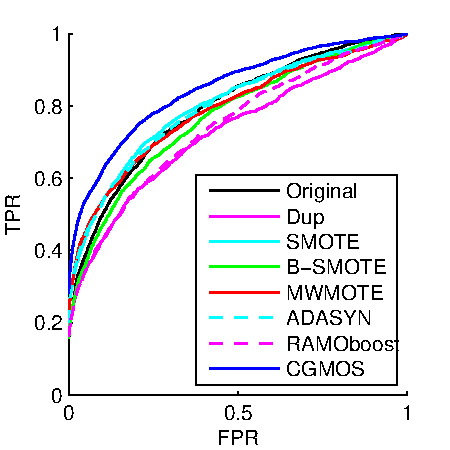
\includegraphics{../Pic/PDF/ROCcurves/nb.pdf}}}
&
\resizebox{0.23\textwidth}{!}{\rotatebox{0}{ 
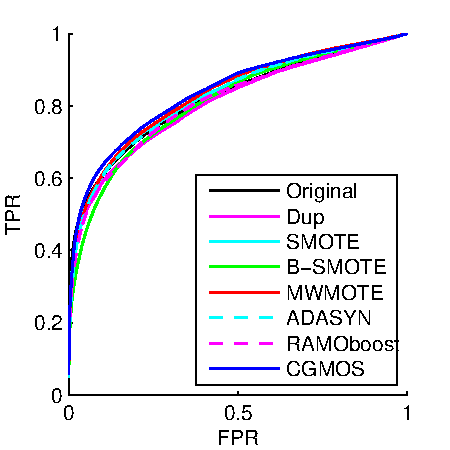
\includegraphics{../Pic/PDF/ROCcurves/knn.pdf}}}
\\
b-kde & knn
\\
\resizebox{0.23\textwidth}{!}{\rotatebox{0}{ 
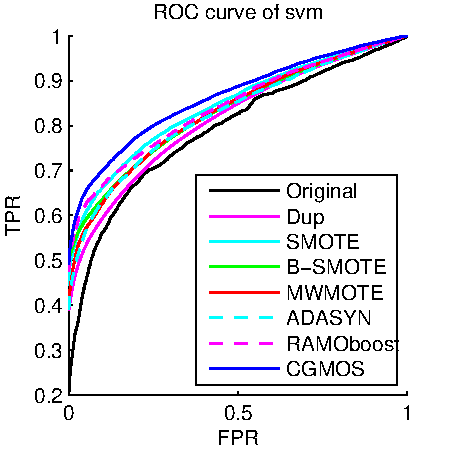
\includegraphics{../Pic/PDF/ROCcurves/svm.pdf}}}
&
\resizebox{0.23\textwidth}{!}{\rotatebox{0}{ 
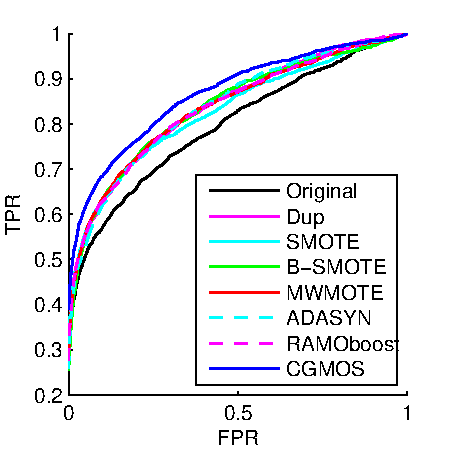
\includegraphics{../Pic/PDF/ROCcurves/nn.pdf}}}
\\
svm & nn
\\
\resizebox{0.23\textwidth}{!}{\rotatebox{0}{ 
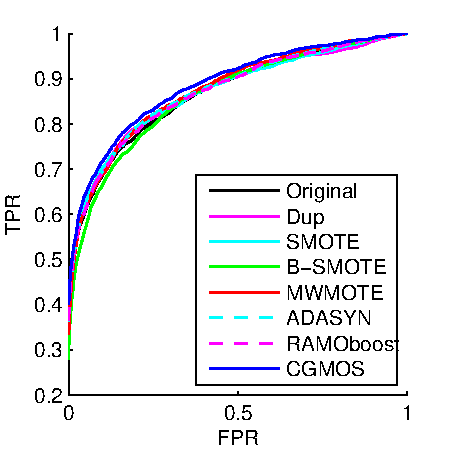
\includegraphics{../Pic/PDF/ROCcurves/rf.pdf}}}
&
\resizebox{0.23\textwidth}{!}{\rotatebox{0}{ 
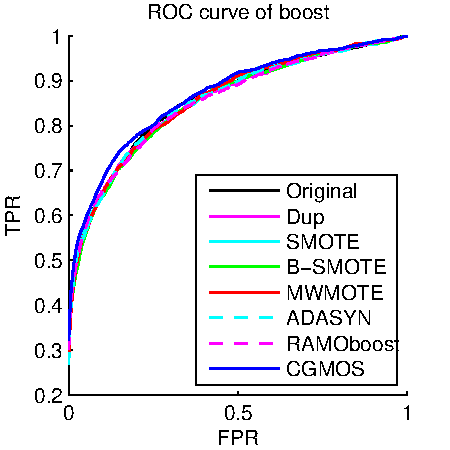
\includegraphics{../Pic/PDF/ROCcurves/boost.pdf}}}
\\
rf & Adaboost.M1
\\
\end{tabular}} 
\caption{ROC curves of real-world data classification results. From left to right, top to bottom, we show the results of 6 different classifiers: b-kde, knn, svm, nn, rf and Adaboost.M1. Curves in blue are the results of the proposed CGMOS.}
\label{fig: real roc} 
\end{figure}

Considering the classification results of the minority class, it can be observed that the proposed approach outperforms most of the compared methods under all classification algorithms in terms of $\fscore$ and $\gscore$. For $\fscore$ and $\gscore$ of the majority class, the proposed approach in most cases is only second to the original data without oversampling. This is because the original dataset is imbalanced and it favors the majority class more than the minority class during classification. Overall, CGMOS achieves the best AUC over all tests. This is because the proposed approach takes into account both of the majority and minority classes and increases the certainties of the two classes while oversampling.

The same conclusion can be made using the ROC curves shown in Fig. \ref{fig: real roc}. The proposed approach has the highest curves almost everywhere. The proposed approach achieves the best result when random forest is used as a classifier. For b-kde as the classifier, the proposed approach gets the largest improvement
since the design of the proposed approach uses b-kde for certainty computations.

To get a closer view of the performances of all compared methods on each dataset, we show the AUC results of CGMOS and all other compared methods for each dataset in Table \ref{tab: results_real_data_per_file}. The table shows that on average the AUC of CGMOS is 2 percent higher than SMOTE whose AUC is 2nd highest. 

Previous studies show that it is not necessary for a learning procedure to obtain best classification results when a dataset is perfectly balanced\cite{batista2004study}\cite{weiss2003learning}. How much to oversample is usually empirically determined \cite{chawla2004editorial}. To evaluate this aspect we performed another experiment in which we synthesized an increasing number of minority samples and investigated how different amounts of new samples impact classification results.

Let $\delta$ denote the difference of data samples between the majority and minority classes. We performed multiple experiments where in each round we synthesized $k\delta$ new samples of the  minority class where $k$ gradually increased from $0.5$ to $5$. The classification results are shown in Figure \ref{fig: increasingnum}. As can be observed in the results, CGMOS achieves the best results in all cases. Also, observe that when increasing the number of data samples added, the results of CGMOS are much more robust compared with other approaches. Note that the results of some methods such as Dup(b-kde), B-SMOTE(knn) and B-SMOTE(Adaboost.M1) are even lower than the results at the starting point where datasets are not oversampled. This highlights the advantage of CGMOS when handling oversampling on boundary samples. 


\begin{table*}[]
\begin{center}
\scalebox{1.0}{
\begin{tabular}{lc!{\VRule[1.5pt]}c|c|c|c!{\VRule[1.5pt]}c|c|c|c!{\VRule[1.5pt]}}
\Cline{1.5pt}{3-10}
 & \textbf{} & \multicolumn{4}{c!{\VRule[1.5pt]}}{\textbf{Minority}} & \multicolumn{4}{c!{\VRule[1.5pt]}}{\textbf{Majority}} \\ \Cline{1.5pt}{2-10} 
\multicolumn{1}{l!{\VRule[1.5pt]}}{} & \textbf{AUC} & \textbf{Precision} & \textbf{Recall} & \textbf{Fscore} & \textbf{Gscore} & \textbf{Precision} & \textbf{Recall} & \textbf{Fscore} & \textbf{Gscore} \\
\specialrule{1.5pt}{0pt}{0pt}
\multicolumn{1}{!{\VRule[1.5pt]}l!{\VRule[1.5pt]}}{\textbf{b-kde}} & &  \multicolumn{4}{c!{\VRule[1.5pt]}}{} & \multicolumn{4}{c!{\VRule[1.5pt]}}{}  \\               
\specialrule{1.5pt}{0pt}{0pt}                     
\multicolumn{1}{!{\VRule[1.5pt]}l!{\VRule[1.5pt]}}{\textbf{Original}} & 0.797 & 0.139 & 0.033 & 0.054 & 0.068 & 0.830 & \textbf{0.995} & \textbf{0.905} & \textbf{0.909}  \\ \hline
\multicolumn{1}{!{\VRule[1.5pt]}l!{\VRule[1.5pt]}}{\textbf{Dup}} & 0.733 & 0.385 & 0.454 & 0.417 & 0.418 & 0.869 & 0.742 & 0.801 & 0.803  \\ \hline
\multicolumn{1}{!{\VRule[1.5pt]}l!{\VRule[1.5pt]}}{\textbf{SMOTE}} & 0.807 & 0.488 & 0.705 & 0.577 & \textbf{0.587} & 0.833 & 0.644 & 0.726 & 0.733  \\ \hline
\multicolumn{1}{!{\VRule[1.5pt]}l!{\VRule[1.5pt]}}{\textbf{B-SMOTE}} & 0.774 & 0.258 & 0.456 & 0.330 & 0.343 & 0.846 & 0.671 & 0.748 & 0.754  \\ \hline
\multicolumn{1}{!{\VRule[1.5pt]}l!{\VRule[1.5pt]}}{\textbf{MWMOTE}} & 0.794 & 0.396 & \textbf{0.754} & 0.520 & 0.547 & 0.836 & 0.557 & 0.669 & 0.682  \\ \hline
\multicolumn{1}{!{\VRule[1.5pt]}l!{\VRule[1.5pt]}}{\textbf{ADASYN}} & 0.802 & 0.395 & 0.632 & 0.487 & 0.500 & 0.817 & 0.598 & 0.691 & 0.699  \\ \hline
\multicolumn{1}{!{\VRule[1.5pt]}l!{\VRule[1.5pt]}}{\textbf{RAMOboost}} & 0.748 & 0.358 & 0.343 & 0.350 & 0.350 & 0.860 & 0.822 & 0.841 & 0.841  \\ \hline
\multicolumn{1}{!{\VRule[1.5pt]}l!{\VRule[1.5pt]}}{\textbf{CGMOS}} & \textbf{0.842} & \textbf{0.536} & 0.517 & \textbf{0.526} & 0.526 & \textbf{0.908} & 0.815 & 0.859 & 0.860  \\ 
\specialrule{1.5pt}{0pt}{0pt}                     
\multicolumn{1}{!{\VRule[1.5pt]}l!{\VRule[1.5pt]}}{\textbf{knn}} & & \multicolumn{4}{c|}{} & \multicolumn{4}{c!{\VRule[1.5pt]}}{}  \\               
\specialrule{1.5pt}{0pt}{0pt}                     
\multicolumn{1}{!{\VRule[1.5pt]}l!{\VRule[1.5pt]}}{\textbf{Original}} & 0.821 & \textbf{0.701} & 0.521 & 0.598 & 0.604 & 0.902 & \textbf{0.942} & \textbf{0.922} & \textbf{0.9217}  \\ \hline
\multicolumn{1}{!{\VRule[1.5pt]}l!{\VRule[1.5pt]}}{\textbf{Dup}} & 0.810 & 0.519 & 0.732 & 0.607 & 0.616 & 0.921 & 0.818 & 0.867 & 0.868  \\ \hline
\multicolumn{1}{!{\VRule[1.5pt]}l!{\VRule[1.5pt]}}{\textbf{SMOTE}} & 0.827 & 0.506 & \textbf{0.804} & 0.621 & 0.638 & 0.925 & 0.805 & 0.861 & 0.863  \\ \hline
\multicolumn{1}{!{\VRule[1.5pt]}l!{\VRule[1.5pt]}}{\textbf{B-SMOTE}} & 0.811 & 0.494 & 0.736 & 0.591 & 0.603 & 0.927 & 0.790 & 0.853 & 0.856  \\ \hline
\multicolumn{1}{!{\VRule[1.5pt]}l!{\VRule[1.5pt]}}{\textbf{MWMOTE}} & 0.832 & 0.504 & 0.792 & 0.616 & 0.632 & \textbf{0.928} & 0.794 & 0.856 & 0.858  \\ \hline
\multicolumn{1}{!{\VRule[1.5pt]}l!{\VRule[1.5pt]}}{\textbf{ADASYN}} & 0.825 & 0.495 & 0.786 & 0.607 & 0.623 & \textbf{0.929} & 0.786 & 0.851 & 0.854  \\ \hline
\multicolumn{1}{!{\VRule[1.5pt]}l!{\VRule[1.5pt]}}{\textbf{RAMOboost}} & 0.827 & 0.540 & 0.684 & 0.604 & 0.608 & 0.918 & 0.847 & 0.881 & 0.881  \\ \hline
\multicolumn{1}{!{\VRule[1.5pt]}l!{\VRule[1.5pt]}}{\textbf{CGMOS}} & \textbf{0.840} & 0.544 & 0.766 & \textbf{0.636} & \textbf{0.646} & 0.925 & 0.842 & 0.882 & 0.883  \\ 
\specialrule{1.5pt}{0pt}{0pt}                     
\multicolumn{1}{!{\VRule[1.5pt]}l!{\VRule[1.5pt]}}{\textbf{svm}} & & \multicolumn{4}{c|}{} & \multicolumn{4}{c!{\VRule[1.5pt]}}{}  \\               
\specialrule{1.5pt}{0pt}{0pt}                     
\multicolumn{1}{!{\VRule[1.5pt]}l!{\VRule[1.5pt]}}{\textbf{Original}} & 0.792 & \textbf{0.632} & 0.587 & 0.609 & 0.609 & 0.882 & 0.935 & 0.908 & 0.908  \\ \hline
\multicolumn{1}{!{\VRule[1.5pt]}l!{\VRule[1.5pt]}}{\textbf{Dup}} & 0.815 & 0.543 & 0.436 & 0.484 & 0.487 & \textbf{0.981} & 0.861 & 0.917 & 0.919  \\ \hline
\multicolumn{1}{!{\VRule[1.5pt]}l!{\VRule[1.5pt]}}{\textbf{SMOTE}} & 0.844 & 0.579 & 0.726 & 0.644 & 0.648 & 0.879 & 0.844 & 0.861 & 0.861  \\ \hline
\multicolumn{1}{!{\VRule[1.5pt]}l!{\VRule[1.5pt]}}{\textbf{B-SMOTE}} & 0.832 & 0.475 & 0.729 & 0.575 & 0.588 & 0.893 & \textbf{0.959} & \textbf{0.924} & \textbf{0.925}  \\ \hline
\multicolumn{1}{!{\VRule[1.5pt]}l!{\VRule[1.5pt]}}{\textbf{MWMOTE}} & 0.830 & 0.547 & 0.647 & 0.593 & 0.595 & 0.880 & 0.884 & 0.882 & 0.882  \\ \hline
\multicolumn{1}{!{\VRule[1.5pt]}l!{\VRule[1.5pt]}}{\textbf{ADASYN}} & 0.827 & 0.536 & 0.654 & 0.589 & 0.592 & 0.880 & 0.755 & 0.813 & 0.815  \\ \hline
\multicolumn{1}{!{\VRule[1.5pt]}l!{\VRule[1.5pt]}}{\textbf{RAMOboost}} & 0.842 & 0.556 & 0.673 & 0.609 & 0.611 & 0.968 & 0.852 & 0.906 & 0.908  \\ \hline
\multicolumn{1}{!{\VRule[1.5pt]}l!{\VRule[1.5pt]}}{\textbf{CGMOS}} & \textbf{0.864} & 0.555 & \textbf{0.788} & \textbf{0.651} & \textbf{0.661} & 0.943 & 0.830 & 0.883 & 0.885  \\ 
\specialrule{1.5pt}{0pt}{0pt}                     
\multicolumn{1}{!{\VRule[1.5pt]}l!{\VRule[1.5pt]}}{\textbf{nn}} & & \multicolumn{4}{c|}{} & \multicolumn{4}{c!{\VRule[1.5pt]}}{}  \\               
\specialrule{1.5pt}{0pt}{0pt}                     
\multicolumn{1}{!{\VRule[1.5pt]}l!{\VRule[1.5pt]}}{\textbf{Original}} & 0.801 & \textbf{0.632} & 0.412 & 0.499 & 0.510 & 0.892 & \textbf{0.962} & \textbf{0.925} & \textbf{0.9258}  \\ \hline
\multicolumn{1}{!{\VRule[1.5pt]}l!{\VRule[1.5pt]}}{\textbf{Dup}} & 0.843 & 0.543 & 0.777 & 0.639 & 0.650 & 0.926 & 0.819 & 0.869 & 0.871  \\ \hline
\multicolumn{1}{!{\VRule[1.5pt]}l!{\VRule[1.5pt]}}{\textbf{SMOTE}} & 0.840 & 0.555 & 0.750 & 0.638 & 0.645 & 0.921 & 0.820 & 0.868 & 0.869  \\ \hline
\multicolumn{1}{!{\VRule[1.5pt]}l!{\VRule[1.5pt]}}{\textbf{B-SMOTE}} & 0.841 & 0.475 & 0.779 & 0.590 & 0.608 & 0.924 & 0.802 & 0.859 & 0.861  \\ \hline
\multicolumn{1}{!{\VRule[1.5pt]}l!{\VRule[1.5pt]}}{\textbf{MWMOTE}} & 0.841 & 0.547 & 0.778 & 0.642 & 0.652 & 0.927 & 0.812 & 0.866 & 0.867  \\ \hline
\multicolumn{1}{!{\VRule[1.5pt]}l!{\VRule[1.5pt]}}{\textbf{ADASYN}} & 0.842 & 0.536 & \textbf{0.786} & 0.637 & 0.649 & 0.929 & 0.803 & 0.861 & 0.863  \\ \hline
\multicolumn{1}{!{\VRule[1.5pt]}l!{\VRule[1.5pt]}}{\textbf{RAMOboost}} & 0.841 & 0.556 & 0.743 & 0.636 & 0.643 & 0.919 & 0.830 & 0.872 & 0.873  \\ \hline
\multicolumn{1}{!{\VRule[1.5pt]}l!{\VRule[1.5pt]}}{\textbf{CGMOS}} & \textbf{0.865} & 0.579 & 0.750 & \textbf{0.653} & \textbf{0.659} & \textbf{0.933} & 0.845 & 0.887 & 0.888  \\ 
\specialrule{1.5pt}{0pt}{0pt}                     
\multicolumn{1}{!{\VRule[1.5pt]}l!{\VRule[1.5pt]}}{\textbf{rf}} & & \multicolumn{4}{c|}{} & \multicolumn{4}{c!{\VRule[1.5pt]}}{}  \\               
\specialrule{1.5pt}{0pt}{0pt}                     
\multicolumn{1}{!{\VRule[1.5pt]}l!{\VRule[1.5pt]}}{\textbf{Original}} & 0.872 & \textbf{0.699} & 0.534 & 0.606 & 0.611 & 0.909 & \textbf{0.956} & \textbf{0.932} & \textbf{0.932}  \\ \hline
\multicolumn{1}{!{\VRule[1.5pt]}l!{\VRule[1.5pt]}}{\textbf{Dup}} & 0.873 & 0.682 & 0.641 & 0.661 & 0.661 & 0.917 & 0.924 & 0.921 & 0.921  \\ \hline
\multicolumn{1}{!{\VRule[1.5pt]}l!{\VRule[1.5pt]}}{\textbf{SMOTE}} & 0.875 & 0.667 & 0.655 & 0.661 & 0.661 & 0.920 & 0.917 & 0.918 & 0.918  \\ \hline
\multicolumn{1}{!{\VRule[1.5pt]}l!{\VRule[1.5pt]}}{\textbf{B-SMOTE}} & 0.867 & 0.653 & 0.637 & 0.645 & 0.645 & 0.920 & 0.906 & 0.913 & 0.913  \\ \hline
\multicolumn{1}{!{\VRule[1.5pt]}l!{\VRule[1.5pt]}}{\textbf{MWMOTE}} & 0.878 & 0.658 & 0.651 & 0.655 & 0.655 & 0.920 & 0.922 & 0.921 & 0.921  \\ \hline
\multicolumn{1}{!{\VRule[1.5pt]}l!{\VRule[1.5pt]}}{\textbf{ADASYN}} & 0.876 & 0.663 & 0.669 & 0.666 & 0.666 & 0.919 & 0.915 & 0.917 & 0.917  \\ \hline
\multicolumn{1}{!{\VRule[1.5pt]}l!{\VRule[1.5pt]}}{\textbf{RAMOboost}} & 0.874 & 0.686 & 0.618 & 0.650 & 0.651 & 0.915 & 0.933 & 0.924 & 0.924  \\ \hline
\multicolumn{1}{!{\VRule[1.5pt]}l!{\VRule[1.5pt]}}{\textbf{CGMOS}} & \textbf{0.884} & 0.685 & \textbf{0.678} & \textbf{0.681} & \textbf{0.681} & \textbf{0.923} & 0.926 & 0.924 & 0.924  \\ 
\specialrule{1.5pt}{0pt}{0pt}                     
\multicolumn{1}{!{\VRule[1.5pt]}l!{\VRule[1.5pt]}}{\textbf{Adaboost.M1}} & & \multicolumn{4}{c|}{} & \multicolumn{4}{c!{\VRule[1.5pt]}}{}  \\               
\specialrule{1.5pt}{0pt}{0pt}                     
\multicolumn{1}{!{\VRule[1.5pt]}l!{\VRule[1.5pt]}}{\textbf{Original}} & 0.868 & \textbf{0.699} & 0.572 & 0.629 & 0.632 & 0.906 & \textbf{0.944} & \textbf{0.925} & \textbf{0.9247}  \\ \hline
\multicolumn{1}{!{\VRule[1.5pt]}l!{\VRule[1.5pt]}}{\textbf{Dup}} & 0.865 & 0.622 & 0.708 & 0.662 & 0.664 & 0.922 & 0.873 & 0.897 & 0.897  \\ \hline
\multicolumn{1}{!{\VRule[1.5pt]}l!{\VRule[1.5pt]}}{\textbf{SMOTE}} & 0.867 & 0.608 & 0.714 & 0.657 & 0.659 & 0.923 & 0.880 & 0.901 & 0.901  \\ \hline
\multicolumn{1}{!{\VRule[1.5pt]}l!{\VRule[1.5pt]}}{\textbf{B-SMOTE}} & 0.864 & 0.581 & 0.724 & 0.644 & 0.648 & \textbf{0.927} & 0.861 & 0.893 & 0.893  \\ \hline
\multicolumn{1}{!{\VRule[1.5pt]}l!{\VRule[1.5pt]}}{\textbf{MWMOTE}} & 0.868 & 0.600 & 0.708 & 0.650 & 0.652 & 0.922 & 0.880 & 0.901 & 0.901  \\ \hline
\multicolumn{1}{!{\VRule[1.5pt]}l!{\VRule[1.5pt]}}{\textbf{ADASYN}} & 0.867 & 0.599 & 0.726 & 0.657 & 0.660 & 0.925 & 0.873 & 0.898 & 0.899  \\ \hline
\multicolumn{1}{!{\VRule[1.5pt]}l!{\VRule[1.5pt]}}{\textbf{RAMOboost}} & 0.865 & 0.631 & 0.699 & 0.663 & 0.664 & 0.922 & 0.882 & 0.901 & 0.902  \\ \hline
\multicolumn{1}{!{\VRule[1.5pt]}l!{\VRule[1.5pt]}}{\textbf{CGMOS}} & \textbf{0.871} & 0.619 & \textbf{0.728} & \textbf{0.670} & \textbf{0.672} & 0.925 & 0.882 & 0.903 & 0.903  \\ 
\specialrule{1.5pt}{0pt}{0pt}
\end{tabular}
}
\end{center}
\caption{A summary of performance measures for the majority and minority classes for all compared methods and real-world datasets.}
\label{tab: results_real_data}
\end{table*}


\begin{table*}[t]
\begin{center}
\scalebox{1.0}{
\centering
\begin{tabular}{!{\VRule[1.5pt]}l!{\VRule[1.5pt]}c|c|c|c|c|c|c|c!{\VRule[1.5pt]}}
\specialrule{1.5pt}{0pt}{0pt} 
 & \textbf{CGMOS} & \textbf{Original} & \textbf{Dup} & \textbf{SMOTE} & \textbf{B-SMOTE} & \textbf{MWMOTE} & \textbf{ADASYN} & \textbf{RAMOboost}\\
 \specialrule{1.5pt}{0pt}{0pt} 
\textbf{BankMarket} & \textbf{0.728} & 0.661 & 0.708 & 0.718 & 0.710 & 0.721 & 0.710 & 0.723 \\ \hline
\textbf{BloodService} & \textbf{0.733} & 0.653 & 0.648 & 0.649 & 0.651 & 0.720 & 0.714 & 0.728 \\ \hline
\textbf{BreastCancer} & 0.992 & 0.992 & \textbf{0.993} & 0.992 & 0.989 & 0.991 & 0.991 & 0.992 \\ \hline
\textbf{BreastTissue} & \textbf{0.984} & 0.899 & 0.946 & 0.932 & 0.917 & 0.937 & 0.908 & 0.943 \\ \hline
\textbf{CarEvaluation} & \textbf{0.997} & 0.995 & 0.845 & \textbf{0.997} & 0.994 & 0.996 & \textbf{0.997} & 0.995 \\ \hline
\textbf{Card'graphy} & \textbf{0.977} & 0.976 & 0.939 & 0.962 & 0.956 & 0.925 & 0.957 & 0.960 \\ \hline
\textbf{CharacterTraj} & 0.985 & 0.962 & 0.717 & 0.985 & 0.978 & 0.981 & \textbf{0.988} & 0.909 \\ \hline
\textbf{Chess} & \textbf{0.977} & 0.974 & 0.959 & 0.973 & \textbf{0.977} & 0.974 & 0.975 & 0.959 \\ \hline
\textbf{ClimateSim} & \textbf{0.908} & \textbf{0.908} & 0.861 & 0.902 & 0.863 & 0.901 & 0.901 & 0.882 \\ \hline
\textbf{Contraceptive} & \textbf{0.724} & 0.705 & 0.699 & 0.712 & 0.702 & 0.705 & 0.702 & 0.705 \\ \hline
\textbf{Fertility} & \textbf{0.673} & 0.615 & 0.594 & 0.634 & 0.592 & 0.604 & 0.639 & 0.638 \\ \hline
\textbf{Haberman} & \textbf{0.651} & 0.623 & 0.577 & 0.600 & 0.593 & 0.594 & 0.587 & 0.586 \\ \hline
\textbf{ILPD} & 0.707 & 0.687 & 0.693 & \textbf{0.715} & 0.703 & 0.702 & 0.693 & 0.703 \\ \hline
\textbf{ImgSeg} & \textbf{0.999} & 0.998 & \textbf{0.999} & 0.997 & 0.998 & 0.998 & 0.997 & 0.998 \\ \hline
\textbf{Leaf} & \textbf{0.908} & 0.880 & 0.782 & 0.852 & 0.775 & 0.836 & 0.839 & 0.821 \\ \hline
\textbf{Libras} & \textbf{0.945} & 0.922 & 0.859 & 0.929 & 0.886 & 0.936 & 0.923 & 0.883 \\ \hline
\textbf{MultipleFs} & \textbf{0.998} & \textbf{0.998} & 0.997 & \textbf{0.998} & 0.997 & 0.997 & 0.996 & 0.997 \\ \hline
\textbf{Parkinson} & 0.841 & 0.676 & 0.692 & 0.834 & 0.791 & 0.837 & \textbf{0.842} & 0.760 \\ \hline
\textbf{PlanRelax} & 0.472 & 0.457 & 0.494 & 0.469 & 0.445 & 0.467 & \textbf{0.488} & 0.464 \\ \hline
\textbf{QSAR} & \textbf{0.901} & 0.886 & 0.879 & 0.895 & 0.863 & 0.886 & 0.886 & 0.882 \\ \hline
\textbf{SPECT} & \textbf{0.820} & 0.772 & 0.803 & 0.808 & 0.811 & 0.752 & 0.801 & 0.799 \\ \hline
\textbf{SPECTF} & 0.819 & 0.819 & 0.800 & 0.805 & 0.816 & 0.812 & \textbf{0.825} & 0.795 \\ \hline
\textbf{SeismicBumps} & \textbf{0.743} & 0.735 & 0.712 & 0.727 & 0.740 & 0.732 & 0.715 & 0.691 \\ \hline
\textbf{Statlog} & \textbf{0.998} & 0.992 & 0.996 & \textbf{0.998} & 0.990 & 0.996 & 0.976 & 0.996 \\ \hline
\textbf{PlatesFaults} & \textbf{0.956} & 0.928 & 0.844 & 0.954 & 0.920 & 0.943 & \textbf{0.956} & 0.881 \\ \hline
\textbf{TAEvaluation} & \textbf{0.748} & 0.682 & 0.644 & 0.703 & 0.671 & 0.707 & 0.665 & 0.657 \\ \hline
\textbf{UserKnowledge} & \textbf{0.958} & 0.837 & 0.919 & 0.953 & 0.947 & 0.951 & 0.950 & 0.888 \\ \hline
\textbf{Vertebral} & \textbf{0.890} & 0.839 & 0.869 & 0.855 & 0.829 & 0.860 & 0.794 & 0.872 \\ \hline
\textbf{Customers} & \textbf{0.952} & 0.930 & 0.943 & 0.946 & 0.884 & 0.902 & 0.946 & \textbf{0.952} \\ \hline
\textbf{Yeast} & \textbf{0.925} & 0.792 & 0.844 & 0.907 & 0.898 & 0.900 & 0.906 & 0.851 \\
\specialrule{1.5pt}{0pt}{0pt} 
\textbf{Average} & \textbf{0.864} & 0.827 & 0.808 & 0.844 & 0.830 & 0.842 & 0.842 & 0.830 \\
\specialrule{1.5pt}{0pt}{0pt} 
\end{tabular}
}
\end{center}
\caption{A summary of AUC of 8 oversampling algorithms over all 30 datasets used in our evaluation. The AUC is averaged over all 6 base classifiers used in the evaluation. It could be observed from above table that CGMOS achieves best AUC measures for 24 datasets out of 30. On average, the AUC of CGMOS is $2\%$ higher than that of the compared approaches.}
\label{tab: results_real_data_per_file}
\end{table*} 

\begin{figure}[ht]
\centerline{ %
\begin{tabular}{ccc}
\resizebox{0.23\textwidth}{!}{\rotatebox{0}{ 
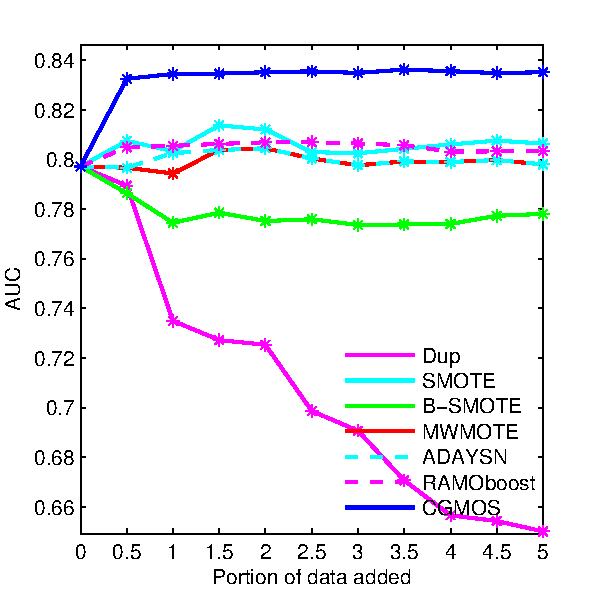
\includegraphics{../Pic/PDF/IncreasingNum/auc/nb.pdf}}}
&
\resizebox{0.23\textwidth}{!}{\rotatebox{0}{ 
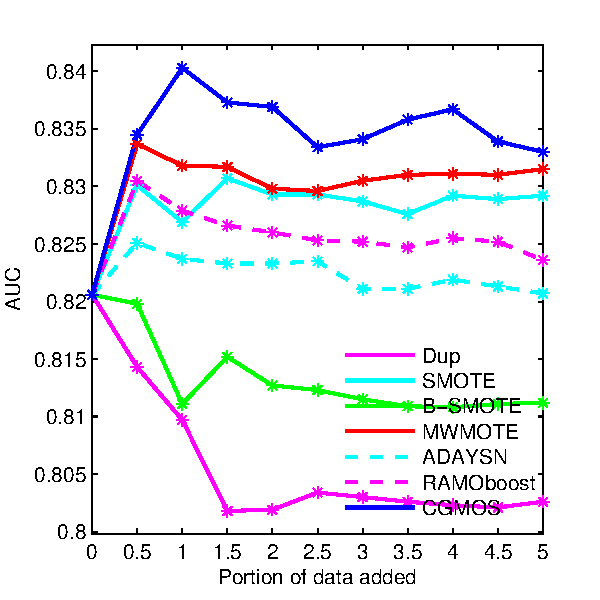
\includegraphics{../Pic/PDF/IncreasingNum/auc/knn.pdf}}}
\\
b-kde & knn
\\
\resizebox{0.23\textwidth}{!}{\rotatebox{0}{ 
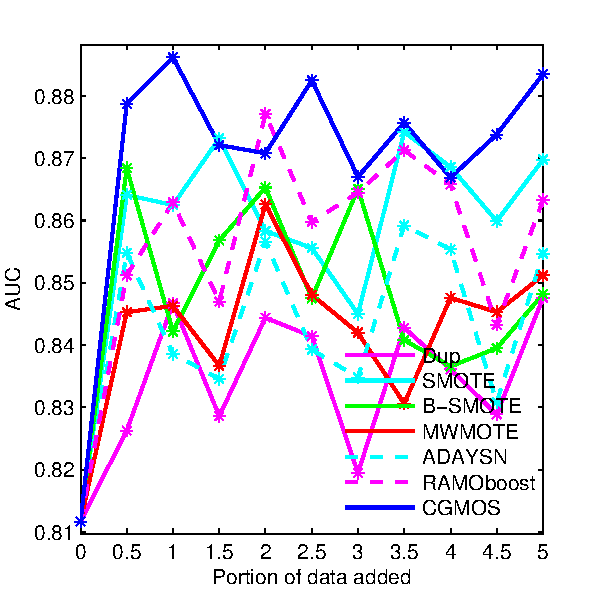
\includegraphics{../Pic/PDF/IncreasingNum/auc/svm.pdf}}}
&
\resizebox{0.23\textwidth}{!}{\rotatebox{0}{ 
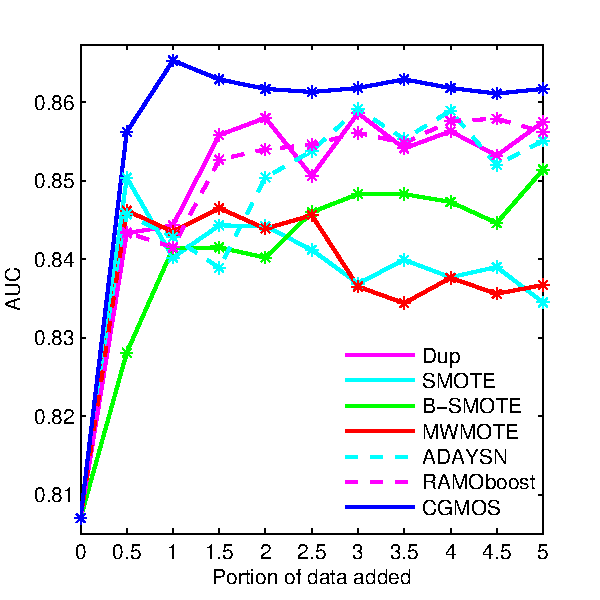
\includegraphics{../Pic/PDF/IncreasingNum/auc/nn.pdf}}}
\\
svm & nn
\\
\resizebox{0.23\textwidth}{!}{\rotatebox{0}{ 
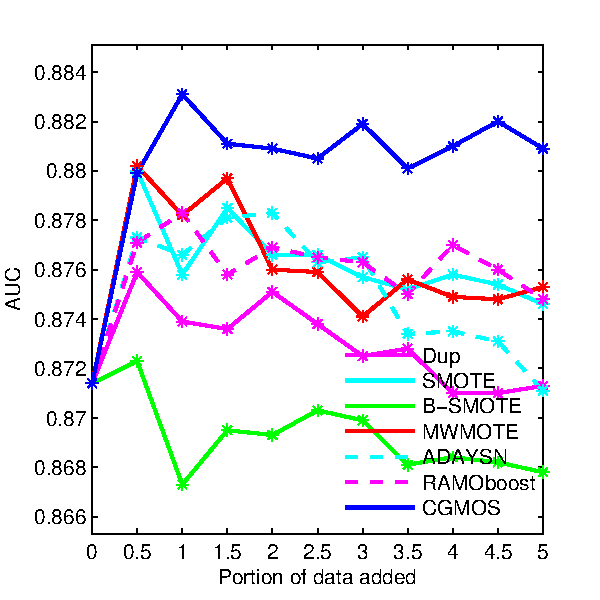
\includegraphics{../Pic/PDF/IncreasingNum/auc/rf.pdf}}}
&
\resizebox{0.23\textwidth}{!}{\rotatebox{0}{ 
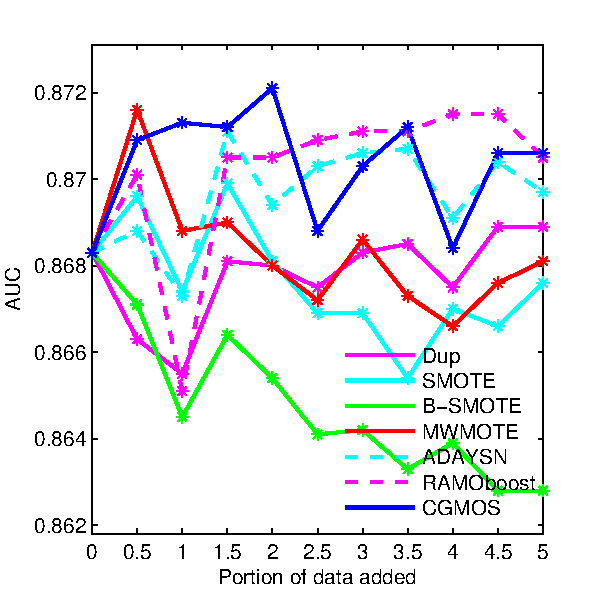
\includegraphics{../Pic/PDF/IncreasingNum/auc/boost.pdf}}}
\\
rf & boost
\\
\end{tabular}} 
\caption{Comparison of results when increasing the number of data synthesized for the minority class. The curves measure the average AUC of the ROC curves. Curves in blue are the results of the proposed CGMOS.}
\label{fig: increasingnum} 
\end{figure} 

\subsection{Statistical Significance Analysis}
We evaluate the statistical significance of the classification results of all compared approaches. We select as the null hypothesis the general statement that sample observations result purely from chance. For the null hypothesis to be rejected as false, the result has to be identified as being statistically significant.

To determine whether to reject a null hypothesis, a $p$-value is calculated, which is the probability of observing an effect given that the null hypothesis is true \cite{JLD:11}. The null hypothesis is rejected if $p$-value is less than the significance level. The significance level is the probability of rejecting the null hypothesis given that it is true. The lower the significance level the more confident we can be in replicating the results and usually the significance level is set at $5\%$. A sample observation is determined to be statistically significant if $p$-value is less than $5\%$, which is formally written as $p<0.05$ \cite{SM:06}.

\textcolor{red}{Usually a statistical hypothesis test is done using $t$-test \cite{BF:08}\cite{zimmerman1997teacher}\cite{demvsar2006statistical}. $t$-test is used to determin if two sets of data are significant from each other, and is most commonly applied when the test statistic would follow a normal distribution. However, for our experiment results which are discrete, they do not necessarily follow a normal distribution. So, instead of testing our hypothesis using $t$-test, we follow the same protocols used in \cite{chen2010ramoboost}\cite{barua2014mwmote} and choose to use Wilcoxon signed-ranks test in this paper. Wilcoxon signed-ranks test is a nonparametric statistical procedure for comparing two samples that are paired, or related \cite{GC09}. Different from $t$-test whose null hypothesis is that the mean difference between pairs is zero, the null hypothesis of Wilcoxon signed-ranks test is that the median difference between pairs of observations is zero.}

\begin{table}
\begin{center}
\scalebox{0.9}{
\begin{tabular}{!{\VRule[1.5pt]}l!{\VRule[1.5pt]}c|c|c|c|c|c!{\VRule[1.5pt]}}
\specialrule{1.5pt}{0pt}{0pt} 
 & \makebox[3em]{\textbf{Knn}} & \makebox[3em]{\textbf{Rf}}& \makebox[3em]{\textbf{B-kde}} & \makebox[3em]{\textbf{Nn}} & \makebox[3em]{\textbf{Svm}} & \makebox[3em]{\textbf{Boost}}\\
\specialrule{1.5pt}{0pt}{0pt} 
\textbf{Original} & 5e-5 & 1e-4 & 0.004 & 1e-4 & 0.026 & 0.04\\\hline
\textbf{Dup} & 2e-6 & 5e-5 & 3e-6 & 0.03 & 0.049 & 0.004\\\hline
\textbf{SMOTE} & 0.003 & 2e-4 & 6e-6 & 0.018 & 0.006 & 0.046\\\hline
\textbf{B-SMOTE} & 4e-6 & 7e-6 & 2e-5 & 5e-4 & 0.047 & 5e-4\\\hline
\textbf{MWMOTE} & 0.046 & 4e-5 & 1e-5 & 0.003 & 0.005 & 0.007\\\hline
\textbf{ADASYN} & 8e-6 & 7e-5 & 9e-5 & 0.005 & 1e-4 & 0.003\\\hline
\textbf{RAMOboost} & 2e-6 & 5e-5 & 3e-6 & 0.001 & 0.045 & 0.035\\
\specialrule{1.5pt}{0pt}{0pt} 
\end{tabular}
}
\end{center}
\caption{A summary of $p$-values of statistical significant tests of classification results using CGMOS against each of all the other competitors. }
\label{tab: signrank}
\end{table}

\subsection{Tuning CGMOS Parameters}
\textcolor{red}{There are two parameters which are tunable in CGMOS. The first one is $\sigma$ used in Eqn.\ref{eqn: sigma} which basically controls the effective range of the kernel and smoothness of the density function when computing certainty. Another parameter can affect the performance of CGMOS is the number of samples used to interpolating a new sample as discussed in section \ref{sec: synthesis of new data}. In SMOTE only two samples, $v=2$, are used in interpolation of a new sample. We propose to use more samples in the interpolation to improve classification performance. We actually validate this proposal in our experiments and do observe a performance gain when using CGMOS as oversampling technique by increasing $v$ to some higher numbers.}

\textcolor{red}{To get the best CGMOS resutls, we thus tune $\sigma$ by changing its value from $1.5$ to $2.0$ and gradually increase $v$ from $2$ to $5$. We compute average classification results for dataset oversampled by CGMOS for all tested classifiers. The results of all possible $\sigma$ and $v$ combination are plot as bar graphs in Figure \ref{fig: interpolationParams}. It could be seen from the figure that CGMOS almost always achieve the best result when $\sigma=1.8$ among results when fixing $v$. However, $\sigma$ has less impact on the results compared with $v$. There is a larger performance gain when we increase $v$ from $2$ to $v=3$. So, the overall best result are obtained when $\sigma=1.8$ and $v=3$ which are used in all experiments of real-world datasets. For experiments of the artificial datasets, since all artificial samples are created as 2 dimensional points, we keep $\sigma=1.8$ and use $v=2$ in all the tests.   }

\begin{figure}[ht]
\centerline{ %
\begin{tabular}{c}
\resizebox{0.47\textwidth}{!}{\rotatebox{0}{ 
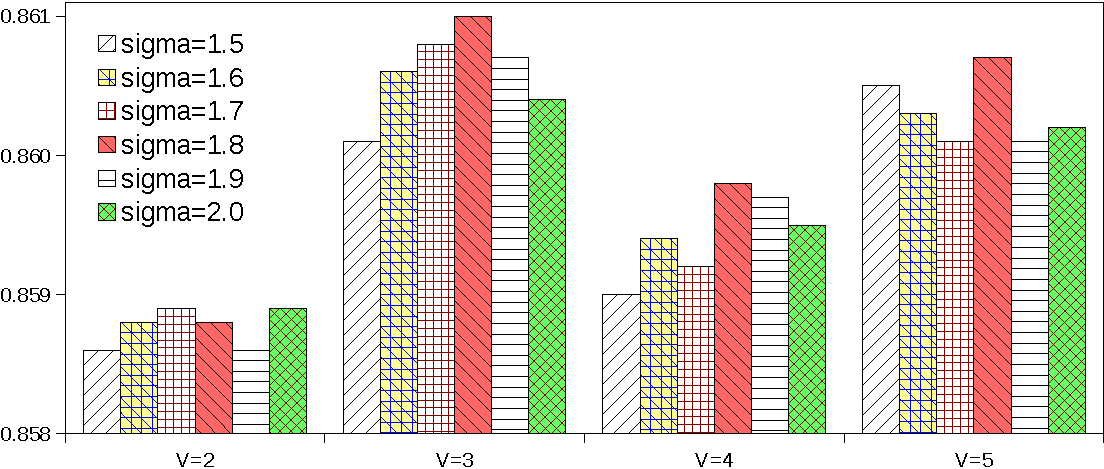
\includegraphics{../Pic/PDF/InterpolationParams/InterpolationHatching.pdf}}}
\end{tabular}} 
\caption{\textcolor{red}{A comparison of AUC results of classifying datasets oversampled by CGMOS using different $\sigma$ in Eqn.\ref{eqn: sigma} and different number of samples in interpolation. To compare with, the results of all other competitors are Original = 0.825, Dup = 0.823, SMOTE = 0.843, B-Smote=0.831, MWMOTE=0.840, ADSYN=0.840 and RAMOboost=0.833.}}
\label{fig: interpolationParams} 
\end{figure} 

\section{Conclusion}
In this paper, we address the imbalanced binary classification problem by proposing a novel minority oversampling strategy. Different from existing approaches, CGMOS does not randomly synthesize new data along decision boundaries. Instead, CGMOS computes the Bayes classification certainties for both the majority and minority classes and then synthesize new samples based on improvement of the certainties for samples in both classes. We prove that CGMOS can achieve better classification results compared with SMOTE. In addition, experimental results show that CGMOS outperforms known oversampling techniques using various metrics.



% use section* for acknowledgment
\ifCLASSOPTIONcompsoc
  % The Computer Society usually uses the plural form
  \section*{Acknowledgments}
\else
  % regular IEEE prefers the singular form
  \section*{Acknowledgment}
\fi


The authors would like to thank...


% Can use something like this to put references on a page
% by themselves when using endfloat and the captionsoff option.
\ifCLASSOPTIONcaptionsoff
  \newpage
\fi



% trigger a \newpage just before the given reference
% number - used to balance the columns on the last page
% adjust value as needed - may need to be readjusted if
% the document is modified later
%\IEEEtriggeratref{8}
% The "triggered" command can be changed if desired:
%\IEEEtriggercmd{\enlargethispage{-5in}}

% references section

% can use a bibliography generated by BibTeX as a .bbl file
% BibTeX documentation can be easily obtained at:
% http://mirror.ctan.org/biblio/bibtex/contrib/doc/
% The IEEEtran BibTeX style support page is at:
% http://www.michaelshell.org/tex/ieeetran/bibtex/
%\bibliographystyle{IEEEtran}
% argument is your BibTeX string definitions and bibliography database(s)
%\bibliography{IEEEabrv,../bib/paper}
%
% <OR> manually copy in the resultant .bbl file
% set second argument of \begin to the number of references
% (used to reserve space for the reference number labels box)
{\small
\bibliographystyle{IEEEtran}
\bibliography{mybib}
}


% biography section
% 
% If you have an EPS/PDF photo (graphicx package needed) extra braces are
% needed around the contents of the optional argument to biography to prevent
% the LaTeX parser from getting confused when it sees the complicated
% \includegraphics command within an optional argument. (You could create
% your own custom macro containing the \includegraphics command to make things
% simpler here.)
%\begin{IEEEbiography}[{\includegraphics[width=1in,height=1.25in,clip,keepaspectratio]{mshell}}]{Michael Shell}
% or if you just want to reserve a space for a photo:

\begin{IEEEbiography}{ }
Biography text here.
\end{IEEEbiography}

% if you will not have a photo at all:
\begin{IEEEbiographynophoto}{ }
Biography text here.
\end{IEEEbiographynophoto}

% insert where needed to balance the two columns on the last page with
% biographies
%\newpage

\begin{IEEEbiographynophoto}{ }
Biography text here.
\end{IEEEbiographynophoto}

% You can push biographies down or up by placing
% a \vfill before or after them. The appropriate
% use of \vfill depends on what kind of text is
% on the last page and whether or not the columns
% are being equalized.

%\vfill

% Can be used to pull up biographies so that the bottom of the last one
% is flush with the other column.
%\enlargethispage{-5in}



% that's all folks
\end{document}


